\documentclass[
    hyperref={breaklinks},
    xcolor={dvipsnames,table,xcdraw},
    10pt]{beamer}

\usetheme[progressbar=frametitle]{metropolis}
\metroset{block=fill}

\usepackage{natbib}[round]
\renewcommand{\cite}{\citep}

\makeatletter

\setbeamerfont{bibliography entry author}{size=\footnotesize,%
                                          series=\normalfont}
\setbeamerfont{bibliography entry title}{size=\footnotesize,%
                                         series=\bfseries}
\setbeamerfont{bibliography entry location}{size=\footnotesize,%
                                            series=\normalfont}
\setbeamerfont{bibliography entry note}{size=\footnotesize,%
                                        series=\normalfont}

\setbeamerfont{author}{size=\Large}

\setbeamertemplate{title page}{
  \begin{minipage}[b][\paperheight]{\textwidth}
    \vspace*{1cm}
    \ifx\inserttitlegraphic\@empty\else\usebeamertemplate*{title graphic}\fi
    \vfill%
    \ifx\inserttitle\@empty\else\usebeamertemplate*{title}\fi
    \ifx\insertsubtitle\@empty\else\usebeamertemplate*{subtitle}\fi
    \vspace{-0.5cm}
    \usebeamertemplate*{title separator}
    \vspace{-0.75cm}
    \ifx\beamer@shortauthor\@empty\else\usebeamertemplate*{author}\fi
    \ifx\insertdate\@empty\else\usebeamertemplate*{date}\fi
    \ifx\insertinstitute\@empty\else\usebeamertemplate*{institute}\fi
    \vspace{0.5cm}
    \textbf{Jury}\\[0.3em]
    {\footnotesize
    \begin{tabular}{@{}lll}
    %Pr\'{e}sident :     & Pr\'{e}nom NOM & Fonction et \'{e}tablissement d'exercice \\
    Rapporteurs :       & Josiane M{\scriptsize OTHE} & Professeure, Université de Toulouse \\
                        & Patrick P{\scriptsize AROUBEK} & Ingénieur de recherche, Université de Paris-Saclay \\
    Examinateurs :      & Lorraine G{\scriptsize OEURIOT} & Maître de conférences, Université Grenoble Alpes \\
                        & Richard D{\scriptsize UFOUR} & Professeur, Nantes Université \\
    Directrice: & Béatrice D{\scriptsize AILLE} & Professeure, Nantes Université \\
    Encadrant :      & Florian B{\scriptsize OUDIN} & Maître de conférences, Nantes Université \\
    \end{tabular}}
    
    \vspace*{0.3cm}
    
    \hfill{}
    \includegraphics[align=c,height=2em]{logos/UN-noir.png}\hfill{}
    \includegraphics[align=c,trim={10em 5.8em 10em 6em},clip,height=3.5em]{logos/logo_LS2N_bleu.pdf}\hfill{}
    \vspace*{0.3cm}
  \end{minipage}
}
\makeatother

\input{manuscript_setup}

\usepackage{fontspec} % ?
\usepackage{appendixnumberbeamer}
\usepackage[scale=2]{ccicons}
\usepackage[export]{adjustbox} % for trimming picture
\usepackage{graphbox} % for centering pictures
\usepackage{scalefnt}
\usepackage{caption}
\DeclareCaptionLabelFormat{nonum}{#1}
\captionsetup{labelformat=nonum}

\tikzfading
  [name=viesturs fading,
   inner color=transparent!0,
   outer color=transparent!100]

\usepackage{arydshln}

% https://blog.dorian-depriester.fr/latex/tikz/annoter-une-image-avec-tikz
\newenvironment{annotation}[2][]{
	\begin{tikzpicture}[]
		\node[anchor=south west,inner sep=0] (image) at (0,0) {\includegraphics[#1]{#2}};
		\begin{scope}[x={(image.south east)},y={(image.north west)},style={font=\vphantom{Ag}}]
}{
		\end{scope}
	\end{tikzpicture}
}
\def\AnnoSep{0.02}	% Marge entre les annotations et l'image
\newcommand{\BckImg}[2][]{
	\node[anchor=south west,inner sep=0] (image) at (0,0) {\includegraphics[#1]{#2}};
}
\newcommand{\annoLeft}[4][->]{
	\draw[->,#1] (0,#2)++(-\AnnoSep,0) node[anchor=east]{#3} -- (#4);
}
\newcommand{\annoRight}[4][->]{
	\draw[->,#1] (0,#2)++(+\AnnoSep+1,0) node[anchor=west]{#3} -- (#4);
}
\newcommand{\annoUp}[4][->]{
	\draw[->,#1] (#2,0)++(0,\AnnoSep+1) node[anchor=south]{#3} -- (#4);
}
\newcommand{\annoDown}[4][->]{
	\draw[->,#1] (#2,0)++(0,-\AnnoSep) node[anchor=north]{#3} -- (#4);
}
  

%% For table and colors
%https://tex.stackexchange.com/a/378511/240347
\renewcommand<>\cellcolor[1]{\only#2{\beameroriginal\cellcolor{#1}}}
%https://tex.stackexchange.com/a/283965/240347
\renewcommand<>\rowcolor[1]{\only#2{\\[-\normalbaselineskip]\beameroriginal\rowcolor{#1}}}
\newcommand<>\cb[2]{\alt#3{\colorbox{#1}{#2}}{#2}}

\newcommand<>\ccancel[1]{\alt#2{\cancel{#1}}{#1}}

% https://tex.stackexchange.com/a/6155/240347
\tikzset{onslide/.code args={<#1>#2}{%
  \only<#1>{\pgfkeysalso{#2}} 
}}
\tikzstyle{show}=[opacity=1]
\tikzstyle{hide}=[opacity=0]

%\newcommand{\fn}[2]{\hl{orange}{#2}}

\setbeamertemplate{section in toc}[sections numbered]
\AtBeginSection[ ]
{
%\begin{frame}
%\sectionpage
%\end{frame}
\begin{frame}{Plan}
    \sectionpage
    %\tableofcontents[hideallsubsections, currentsection,subsectionstyle=show/show/hide]
\end{frame}
}


\title{Indexation de bout-en-bout dans les bibliothèques numériques scientifiques}
\subtitle{}
\date{28/03/2022}
\author{Ygor \textsc{Gallina}}
%\institute{Université de Nantes, LS2N}


\begin{document}

\maketitle

\section*{Introduction}

\begin{frame}{Bibliothèques numériques scientifiques}
    % Il existe plusieurs bibliothèques num sci en fonction des domaines
    % Leur taille croît exponentiellement
    \begin{tikzpicture}
    
        \node (pubmed) {
        \includegraphics[width=.47\textwidth]{figures/pic_dl/contexte_pubmed.png}
        };
        \node<2>[fill opacity=.85, text opacity=1, fill=white, align=center,text width=2.5cm] at (pubmed) {PubMed \\ Bio-médical \\ 24\,566\,348 doc.};
        
        \node[right=.5cm of pubmed] (arxiv) {
        \includegraphics[width=.47\textwidth,trim=0 9em 0 0, clip]{figures/pic_dl/contexte_arxiv.png}
        };
        \node<2>[fill opacity=.75, text opacity=1, fill=white, align=center,text width=3cm] at (arxiv) {arXiv \\ Sciences formelles \\ 1\,999\,642 doc.};
    
        \node[below=.5cm of pubmed] (acmdl) {
        \includegraphics[width=.47\textwidth]{figures/pic_dl/contexte_acm_dl.png}
        };
        \node<2>[fill opacity=.75, text opacity=1, fill=white, align=center,text width=2.5cm] at (acmdl) {ACMDL\\ Informatique  \\ 654\,532 doc.};
        
        \node[right=.5cm of acmdl] (acl) {
        \includegraphics[width=.47\textwidth, trim=0 10em 0 0, clip]{figures/pic_dl/contexte_acl_anthology.png}
        };
        \node<2>[fill opacity=.75, text opacity=1, fill=white, align=center,text width=2.5cm] at (acl) {ACL \\ TALN \\ 74\,432 doc.};
        
        \only<3>{
        \begin{scope}[
            scale=0.4, transform shape]
        \fill[fill opacity=.75, text opacity=1,white] (acmdl.south west) rectangle (acmdl.north east);
        \fill[fill opacity=.75, text opacity=1,white] (pubmed.south west) rectangle (pubmed.north east);
        \fill[fill opacity=.75, text opacity=1,white] (acl.south west) rectangle (acl.north east);
        \fill[fill opacity=.75, text opacity=1,white] (arxiv.south west) rectangle (arxiv.north east);
        
        \pgfplotsset{
            axis x line=bottom, axis y line=left,
            enlargelimits=true,
            xlabel={Année}, ylabel=\text{Soumissions},
            anchor=center,
            x tick label style={ % remove thousands separator for diplaying years https://tex.stackexchange.com/a/31277/240347
                /pgf/number format/.cd, use comma, 1000 sep={},
            },
            every tick label/.append style={font=\Large},
            xtick={2000,2010,2020},
            scaled y ticks=false, % remove scientific notation from axis (https://tex.stackexchange.com/questions/119887/remove-the-scientific-notation-which-is-unreasonable)
        }
        
        \begin{axis}[
            at={(acmdl)},
            ytick={10000,20000,30000},
            yticklabels={10K,20K,30K}]
        \addplot+[smooth] coordinates {
        (1995,6084)(1996,6787)(1997,6942)(1998,7798)(1999,7447)(2000,9096)(2001,8676)(2002,11420)(2003,12994)(2004,15356)(2005,17708)(2006,19777)(2007,20685)(2008,22411)(2009,24403)(2010,27503)(2011,26591)(2012,27302)(2013,26271)(2014,27480)(2015,27498)(2016,28887)(2017,30837)(2018,32890)(2019,35286)(2020,32778)
        %(1995, 43642)(1996, 47134)(1997, 51372)(1998, 50508)(1999, 53524)(2000, 57547)(2001, 57581)(2002, 63690)(2003, 58281)(2004, 66721)(2005, 100763)(2006, 119920)(2007, 120407)(2008, 133729)(2009, 175313)(2010, 146084)(2011, 137865)(2012, 134483)(2013, 112786)(2014, 104140)(2015, 124040)(2016, 117497)(2017, 93819)(2018, 80789)(2019, 81798)(2020, 96451)%(2021, 51069)(2022, 3542)
        };
        \end{axis}
        
        \begin{axis}[
            at={(pubmed)},
            ytick={500000,1000000,1500000},
            yticklabels={{0,5M},1M,{1,5M}}
            ]
        \addplot+[smooth] coordinates {
        (1995, 449050)(1996, 458678)(1997, 456812)(1998, 474666)(1999, 493712)(2000, 532503)(2001, 547504)(2002, 565256)(2003, 594340)(2004, 639530)(2005, 700229)(2006, 749769)(2007, 786530)(2008, 836935)(2009, 877310)(2010, 941684)(2011, 1019685)(2012, 1088548)(2013, 1148929)(2014, 1203202)(2015, 1254639)(2016, 1280910)(2017, 1297742)(2018, 1338381)(2019, 1397240)(2020, 1617944)};
        \end{axis}

        \begin{axis}[
            at={(acl)},
            ytick={2000,4000,6000},
            yticklabels={2K,4K,6K}
            ]
        \addplot+[smooth] coordinates {
        (1995, 386)(1996, 619)(1997, 668)(1998, 1099)(1999, 543)(2000, 1254)(2001, 814)(2002, 1216)(2003, 1186)(2004, 1924)(2005, 1261)(2006, 2149)(2007, 1578)(2008, 2196)(2009, 2204)(2010, 3053)(2011, 2265)(2012, 3375)(2013, 2795)(2014, 3610)(2015, 2945)(2016, 4166)(2017, 3340)(2018, 4597)(2019, 4947)(2020, 7140)%(2021, 6857)
        };
        \end{axis}
        
        \begin{axis}[
            at={(arxiv)},
            ytick={50000,100000,150000},
            yticklabels={50K,100K,150K}]
        \addplot+[smooth] coordinates {
        %(1991, 306)(1992, 3263)(1993, 6743)(1994, 10097)
        (1995, 13014)(1996, 15866)(1997, 19624)(1998, 24172)(1999, 27704)(2000, 30601)(2001, 33214)(2002, 36121)(2003, 39414)(2004, 43727)(2005, 46855)(2006, 50227)(2007, 55638)(2008, 58915)(2009, 64047)(2010, 70131)(2011, 76578)(2012, 84603)(2013, 92641)(2014, 97517)(2015, 105280)(2016, 113380)(2017, 123523)(2018, 140616)(2019, 155866)(2020, 178329)};
        \end{axis}
        \end{scope}
        \node[text width=5cm, align=center] at ($(acmdl)!.5!(arxiv)$) {\textbf{Nombre de soumissions\\par année}};
        }
        
    \end{tikzpicture}
    
\end{frame}

\iffalse
\begin{frame}{Recherche de document}
    % Plus il y a de document, plus c'est difficile de trouver ce que l'on cherche.
    \begin{figure}
        \centering

        \begin{tikzpicture}[spy using outlines={rounded rectangle,magnification=3,width=2cm,height=1cm,connect spies}]
        \node[anchor=south west,inner sep=0] (image) at (0,0) {\includegraphics[width=.8\textwidth,trim={0 25em 0 0},clip]{figures/res_dl/google_scholar_all.png}};
        %\draw[help lines,xstep=1,ystep=1] (image.south west) grid (image.north east);
        \spy[blue] on (2, 5.67) in node at (5, 5);
        \end{tikzpicture}
    \end{figure}
\end{frame}
\fi

\begin{frame}{Recherche de document}
    % Plus il y a de document, plus c'est difficile de trouver ce que l'on cherche.
    \begin{figure}
        \centering

        \begin{tikzpicture}[spy using outlines={rounded rectangle,height=1cm}]
        
        \node[anchor=south west,inner sep=0] (image1) at (0,0) {\includegraphics[width=.80\textwidth,,trim=0 30em 0 0,clip]{figures/res_dl/context_scholar-1.png}};
        \spy[blue, magnification=2.25, width=10cm] on (2.9, 5.65) in node at (3.55, 5.8);
        \spy[blue, magnification=3, width=2cm, connect spies] on (2.37, 5.1) in node at (4.5, 5);
        
        %\node[anchor=south west,inner sep=0, right= .25 of image1] (image2) %{\includegraphics[width=.49\textwidth]{figures/res_dl/context_scholar-2.png}};
        
        %\draw[help lines,xstep=1,ystep=1] (0,0) grid (image1.north east);
        
        %\draw[green, rounded corners] (0.3,5.1) rectangle (4.5,4.2);
        

        \end{tikzpicture}
    \end{figure}
\end{frame}

%\newcommand{\highall}[1]{\textbf<4,5>{\textcolor<4,5>{color0}{#1}}}
%\newcommand{\highkw}[1]{\textbf<4,5>{\textcolor<4,5>{color0}{#1}}}
    
\begin{frame}{Indexation}
    % Indexation: identifier les descripteur d'un document pour pouvoir effectuer une recherche
    % Manuelle: contrôllée (ou non), chère
    % Automatique: grand rappel, petite précision, titre résumé mots-clés
    
    Représenter un document pour qu'il soit facilement recherchable.
    
    
%     \begin{figure}
%     \centering
%     %\centerfloat
%     \resizebox{0.98\textwidth}{!}{%
%     \begin{tabular}{|p{1.3\textwidth}|}
%     \textbf{Recherche d' informations dans un environnement distribué}
%     \vspace{0.9em}
%     Le Web ou les bibliothèques numériques offrent la possibilité d'interroger de nombreux serveurs d' information (collections ou moteurs de recherche) soulevant l'épineux problème de la sélection des meilleures sources de documents et de la fusion des résultats provenant de différents serveurs interrogés. [\ldots]%Dans cet article, nous présentons un nouvelle approche pour la sélection des collections basée sur les arbres de décision. De plus, nous avons évalué différentes stratégies de fusion et de sélection permettant une meilleure vue d'ensemble des différentes solutions.
%     \vspace{1.1em}
%     \textbf{Mots-clés auteur}: recherche d'information, modèle vectoriel, arbre, arbre de décision, moteur de recherche, indexation
%     \vspace{0.2em}
%     \end{tabular}%
%     }
% \end{figure}
    
    \begin{figure}
        \centering
        \begin{annotation}[width=.7\textwidth]{figures/contexte_catalogue_card.jpg}
        %\draw[help lines,xstep=.1,ystep=.1] (0,0) grid (1,1);
        \annoLeft{.8}{Autrice}{.12,.8}
        \annoLeft{.68}{Titre}{.12,.68}
        \annoLeft{.45}{Résumé}{.12,.45}
        \annoLeft{.27}{Sommaire}{.12,.27}
        %\annoLeft{.1}{Mots-clés}{.12,.17}
        \draw[->] (0,.1)++(-\AnnoSep,0) node[anchor=east,onslide={<2>rounded corners, draw=red, thick}]{Mots-clés} -- (.12,.17);
        \end{annotation}
        
        \caption{\scriptsize Notice scientifique. Source: \href{https://www.libraryhistorybuff.org/catalog-cards.htm}{libraryhistorybuff.org/catalog-cards.htm}}
    \end{figure}
    
\end{frame}

\begin{frame}{Indexation par mots-clés}

    Les mots-clés sont généralement des \textbf{syntagmes nominaux} qui représentent les \textbf{concepts les plus importants} d’un document et servent de \textbf{condensateur textuel}.~\cite{amar_les_1997}

    %\azj
    %Leur intérêt principal est d'enrichir l'indexation.

    \begin{block}{Types d'annotation}
        \begin{itemize}
        \item \textbf{indexeur professionnel} (bibliothèque) 
        \item \textbf{auteur} (conférences / journaux)
        \item \textbf{lecteur} (logiciel gestion bibliographique / étudiant·es)
        \end{itemize}
    \end{block}

    \begin{alertblock}{Coût de l'annotation par des indexeurs}
    %\textbf{Coût de l'annotation par des indexeurs} \\
        $\simeq$10\$/doc dans PubMed \\
        \phantom{\textbf{Coût}:} \alt<2>{\textbf{=> 15 M\$ en 2020} et croissance exponentielle !}{}
    \end{alertblock}

\end{frame}


\iffalse
\begin{frame}{Indexation automatique}
    \begin{figure}
        \centering
        %\centerfloat
    \resizebox{0.98\textwidth}{!}{%
    \begin{tabular}{|p{1.3\textwidth}|}
    \color{black!50}
    \highkw{Grammaires} \highall{factorisées} pour des \highkw{dialectes} \highall{apparentés} \\
    \color{black!50}
    Pour la \highall{formalisation} du \highall{lexique} et de la \highkw{grammaire} de \highkw{dialectes} \highall{étroitement apparentés}, il peut se \highall{révéler utile} de \highall{factoriser} une \highall{partie} du \highall{travail} de \highkw{modélisation}. Les \highall{sous systèmes linguistiques} \highall{isomorphes} dans les \highall{différents} \highkw{dialectes} \highall{peuvent} alors faire l'\highall{objet} d'une \highall{\textcolor<5>{color1}{description commune}}, les \highall{différences} étant \highall{spécifiées} par \highall{ailleurs}. Cette \highall{démarche aboutit} à un \highall{modèle} de \highkw{grammaire} à \highall{couches}: le \highall{noyau} est \highall{commun} à la \highall{famille} de \highkw{dialectes}, et une \highall{couche superficielle} \highall{détermine} les \highall{caractéristiques} de \highall{chacun}. Nous \highall{appliquons} ce \highall{procédé} à la \highall{famille} des \highall{langues créoles} à \highall{base lexicale française} de l'\highall{aire américano-caraïbe}.

    \vspace{0.9em}

    \textbf{Mots-clés auteurs}: \highkw{tag, modélisation, grammaire, variation~dialectale}
    \end{tabular}%
    }
    \caption{Notice scientifique du corpus TALN-Archives (id: {\footnotesize taln-2008-long-016})).}
\end{figure}

    \begin{block}{Indexation automatique \say{plein texte}}
    \only<4-5>{
    \begin{itemize}
        \item titre + résumé + mots-clés (auteur / indexeur)
        \item privilégie le rappel
    \end{itemize}
    }
    \end{block}
\end{frame}
\fi

% #1 number of teeths
% #2 radius intern
% #3 radius extern
% #4 angle from start to end of the first arc
% #5 angle to decale the second arc from the first 
\newcommand{\gear}[5]{%
\foreach \i in {1,...,#1} {%
    [rotate=(\i-1)*360/#1]
        (0:#2) arc (0:#4:#2)
        {[rounded corners=1.5pt] -- (#4+#5:#3) arc (#4+#5:360/#1-#5:#3)}
        -- (360/#1:#2)
}}  

\begin{frame}{Production automatique de mots-clés}

    \begin{figure}
    \centering
    \begin{tikzpicture}

    \node[rounded corners, draw=gray!50!black, fill=gray!50, minimum width=1cm, text width=2.5cm, align=center, minimum height=1cm] (method) at (0,0) {Méthode automatique};
    
    \pic[left=2cm of method, local bounding box=doc] {doc={scale 1.5}};
    \node[below=.5cm of doc] {Document};
    
    \pic[right=2cm of method, local bounding box=kws] {kws={scale 1}};
    \node[below=.5cm of kws] {Mots-clés};
    
    \draw[->] (doc.east) -> (method);
    \draw[->] (method) -> (kws.west);

    \end{tikzpicture}
    \end{figure}
    
    \begin{itemize}
        \item 1972: travaux pionniers (\tfidf~\cite{jones_statistical_1972})
        \item 2000: essor des méthodes extractives
        \item 2017: introduction des méthodes génératives
    \end{itemize}
\end{frame}

\begin{frame}{Jeux de données annotés en mots-clés}
    %\newcommand{\tikzmark}[1]{%  \tikz[overlay,remember picture] \node (#1) {};}

%https://tex.stackexchange.com/a/6250/240347
%\alt<3>{\newcolumntype{C}{>{\columncolor{color1!40}}r}}{\newcolumntype{C}{r}}

\begin{table}[htbp!]
\centering
\resizebox{0.8\textwidth}{!}{
    \begin{tabular}{crcccrr}%rr}
    \cmidrule[1pt]{2-7}
        &
        \textbf{Corpus} &
        \textbf{Lang.} &
        \textbf{Ann.} &
        \textbf{\#Entr.} &
        \textbf{\#Test} &
        \textbf{\#mots} \\
        %& \textbf{\#mc} & \textbf{\%abs} \\
    \cmidrule[.5pt]{2-7}
    %\tikzmark{b}
    \rowcolor<2>{color1!40}
    & \cellcolor<3>{color1!40} CSTR~\cite{witten_kea:_1999}              & en & $A$        & \cellcolor<3>{color1!40} 130 & 500 &11501 \\% & 5 & 19 \\
    \rowcolor<2>{color1!40}
    & NUS~\cite{goh_keyphrase_2007}             & en & $A \cup L$ & -   & 211 & 8398 \\% &11 & 14 \\
    \rowcolor<2>{color1!40}
    & PubMed~\cite{schutz_keyphrase_2008}       & en & $A$        & -   & 1320& 5323 \\% & 5 & 17 \\
    \rowcolor<2>{color1!40}
    & ACM~\cite{krapivin_large_2009}            & en & $A$        & -   & 2304& 9198 \\% & 5 & 16 \\
    \rowcolor<2>{color1!40}
    \multirow{-5}{*}[-0.4ex]{\rotatebox{90}{\textbf{Articles}}}
    & Citeulike-180~\cite{medelyan_human-competitive_2009} & en & $L$ & -&182 & 8590 \\% & 5 & 11 \\
    \rowcolor<2>{color1!40}
    & \cellcolor<3>{color1!40} SemEval-2010~\cite{kim_semeval-2010_2010} & en & $A \cup L$ & \cellcolor<3>{color1!40} 144 & 100 & 7961 \\% &15 & 20 \\
    
    %\cmidrule{7-9} %\vspace{-.5em}
    %\multirow{-6}{*}[-0.4ex]{\rotatebox{90}{\textbf{Articles}}}
    %& & & & & \textbf{Avg.} & 8495  & 8  & 16 \\
    
        \cmidrule[.5pt]{2-7}
    
    %\tikzmark{a}
    \rowcolor<2>{color1!40}
    & \cellcolor<3>{color1!40} Inspec~\cite{hulth_improved_2003}         & en & $I$ & \cellcolor<3>{color1!40} 1\,000  & 500    & 135 \\% & 10 & 22 \\
    \rowcolor<2>{color1!40}
    & KDD~\cite{caragea_citation-enhanced_2014} & en & $A$ & -       & 755    & 191 \\% &  4 & 49 \\
    \rowcolor<2>{color1!40}
    & WWW~\cite{caragea_citation-enhanced_2014} & en & $A$ & -       & 1\,330 & 164 \\% &  5 & 52 \\
    \rowcolor<2>{color1!40}
    & TermITH-Eval~\cite{bougouin_termith-eval:_2016} & fr & $I$ & - & 400    & 165 \\% & 12 & 60 \\
    \rowcolor<2>{color1!40}
    \multirow{-5}{*}[-0.4ex]{\rotatebox{90}{\textbf{Notices}}}
    & \cellcolor<3>{color1!60} \textbf<3>{KP20k~\cite{meng_deep_2017}}               & en & $A$ & \cellcolor<3>{color1!60} \textbf<3>{530\,K}  & 20\,K  & 176 \\% &  5 & 43 \\
    %OAGK~\cite{cano_keyphrase_2019-1}         & en & $A$ & 23\,M   & -      & ?   & ?    & ? \\
    %\cmidrule{7-9} %\vspace{-.5em}
    %\multirow{-6}{*}[-0.4ex]{\rotatebox{90}{\textbf{Notices}}}
    %& & & & & \textbf{Avg.} & 166  & 7  & 45 \\
    
    
    \cmidrule[.5pt]{2-7}
    %Reuters-21578~\cite{hulth-megyesi:2006:COLACL}     & en & \\
    %110-PT-BN-KP~\cite{marujo_keyphrase_2011} & pt & $L$ & 100 & 10 & 439 & 27.6 & 7.5 \\
    & DUC-2001~\cite{wan_single_2008}            & en & $L$ & -    & 308 & 847 \\% &  8 &  4 \\
    & \cellcolor<3>{color1!40} 500N-KPCrowd~\cite{marujo_supervised_2012} & en & $L$ & \cellcolor<3>{color1!40} 450  &  50 & 465 \\% & 46 & 11 \\
    \multirow{-4}{*}[-0.4ex]{\rotatebox{90}{\textbf{Journalistique}}}
    & Wikinews~\cite{bougouin_topicrank:_2013}   & fr & $L$ & -    & 100 & 314 \\% & 10 & 11 \\
    %\rowcolor<3>{color1!40}
    %& KPTimes~\cite{gallina_kptimes_2019}        & en & $E$ &\textbf<3>{260\,K}&20\,K& 784 &  5 & 41 \\

    %\cmidrule{7-9} %\vspace{-.5em}
    %\multirow{-5}{*}[-0.4ex]{\rotatebox{90}{\textbf{Journalistique}}}
    %& & & & & \textbf{Avg.} & 603  & 17  & 17 \\
    \cmidrule[1pt]{2-7}
    \end{tabular}
    
    %\tikz[right=5cm,overlay,remember picture] \node[rotate=90, anchor=center] at ($(a)!0.5!(b)$) {Notices};
    %\tikz[overlay,remember picture] \draw[-triangle 45] ($(a.north east)+(-0.2,0.2)$) -- ($(b.south west)+(0.3,-0.2)$);
}
%\caption{\footnotesize Statistiques des jeux de données de production automatique de mots-clés.
%Les mots-clés de référence sont annotés par les auteurs ($A$) ou des indexeurs professionnels ($I$).
%La table présente le nombre de documents dans les corpus d'entraînement (\#Entr.) et de test (\#Test) ainsi que le nombre moyen de mots-clés (\#mc), de mots (\#mots) et le ratio de mots-clés absent (\%abs) par document.}
%\label{tab:datasets_abstract}
\end{table}
    
    \begin{itemize}
        \item Majorité de documents scientifiques
        \item Articles pleins peu accessibles (\emph{paywall})
        
    \end{itemize}
\end{frame}

\begin{frame}<1>[label=problematiques]{Objectifs}
    \begin{enumerate}
        \item \textcolor<2,3>{black!30}{Démontrer la validité des méthodes génératives.}
        \only<1>{
        \begin{itemize}
            \item Entraînement sur plusieurs jeux de données
            \item Généralisation à d'autres genres de documents
        \end{itemize}}
        
        \item \textcolor<1,3>{black!30}{Comparer les performances des méthodes état de l'art.}
        \only<2>{
        \begin{itemize}
            \item Cadre expérimental strict et unifié
            \item Influence du type d'annotation sur l'évaluation
            %\item Influence du type d'annotation sur l'entraînement
        \end{itemize}}
        
        \item \textcolor<1,2>{black!30}{\'Evaluer la qualité des mots-clés au travers d'une tâche applicative.}
        \only<3>{
        \begin{itemize}
            \item Nouveau cadre d'évaluation extrinsèque
            \item Évaluation des méthodes état de l'art
        \end{itemize}}
    \end{enumerate}
    
\end{frame}

\begin{frame}[fragile]{Comparaison des performances}
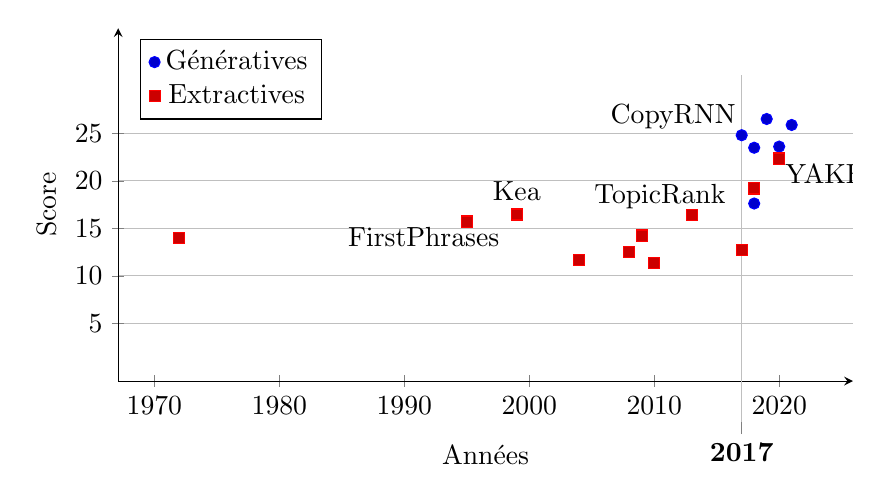
\begin{tikzpicture}
\begin{axis}[
        axis x line=bottom,axis y line = left,enlargelimits=true,
        width=0.9\textwidth,
        height=0.5\textwidth,
        xlabel={Années},
        ylabel={Score},
        ymajorgrids=true,
        ytick={5, 10, 15, 20, 25},
        x tick label style={/pgf/number format/.cd, use comma, 1000 sep={},},
        ymin=2, ymax=33,
        legend pos=north west,
        extra x ticks={2017},
        extra x tick style={grid=major,yshift=-.6cm},
        extra x tick labels={\textbf{2017}}
        ]
\addplot+[only marks] table[meta={end2end}] {
        year mean end2end label
        2017.0 24.82 1 CopyRNN
        2018.0 17.62 1 CorrRNN
        %2018.0 23.76 1 catSeq
        2018.0 23.5 1 catSeqD
        %2019.0 23.52 1 catSeqCorr
        %2019.0 23.98 1 catSeqTG
        2019.0 26.53 1 catSeqTG-2RF1
        2020.0 23.62 1 Transformer
        2021.0 25.9 1 SEG-Net
    };
    \addlegendentry{Génératives}

    \addplot+[only marks] table[meta={end2end}] {
        year mean end2end label
        1972.0 13.96 0 Tf-Idf
        1995.0 15.72 0 FirstPhrases
        1999.0 16.46 0 Kea
        2004.0 11.64 0 TextRank
        %2008.0 10.73 0 ExpandRank
        2008.0 12.49 0 SingleRank
        2009.0 14.24 0 KpMiner
        %2010.0 6.67 0 RAKE
        2010.0 11.34 0 TPR
        2013.0 16.37 0 TopicRank
        2017.0 12.75 0 PositionRank
        2018.0 19.21 0 EmbedRank
        %2018.0 16.57 0 MPRank
        2020.0 22.36 0 YAKE
    };
    \addlegendentry{Extractives}
    \node[inner sep=2pt,anchor=south west] at (axis cs:1972,13.96) {\tfidf};
    \node[inner sep=2pt,anchor=20] at (axis cs:1995,15.72) {FirstPhrases};
    \node[inner sep=2pt,anchor=south east] at (axis cs:2017,24.82) {CopyRNN};
    \node[inner sep=5pt,anchor=south] at (axis cs:1999,16.46) {Kea};
    \node[inner sep=2pt,anchor=north west] at (axis cs:2020,22.36) {YAKE!};
    \node[inner sep=2pt,anchor=330] at (axis cs:2013,16.37) {TopicRank};

\end{axis}
\end{tikzpicture}

Grande diversité de métrique et jeux de données utilisés.

Moyenne des scores rapportés de \textbf{toutes métriques et jeux de données confondus}.

\end{frame}

\begin{frame}[fragile]{Comparaison des performances}
\begin{tikzpicture}
\begin{axis}[
        axis x line=bottom,axis y line = left,enlargelimits=true,
        width=0.9\textwidth, height=0.5\textwidth,
        xlabel={Années}, ylabel={F@5},
        ymajorgrids=true,
        ytick={5, 10, 15, 20, 25},
        x tick label style={/pgf/number format/.cd, use comma, 1000 sep={},},
        ymin=2, ymax=33,
        legend pos=north west,
        extra x ticks={2017},
        extra x tick style={grid=major,yshift=-.6cm},
        extra x tick labels={\textbf{2017}}
        ]
        
    \addlegendimage{mark=*, color=white, fill=color2}
    \addlegendentry{SemEval-2010}
    \addlegendimage{mark=*, color=white, fill=color3}
    \addlegendentry{Inspec}

    \addplot[only marks, mark=*, every mark/.append style={color=white,fill=color2}
    ] table {
        year mean end2end label
        2017 29.23 * CopyRNN
        2018 32.0 * CorrRNN
        2018 24.3 * catSeqD
        2019 28.7 * catSeqTG-2RF1
        2020 25.1 * Transformer
        2021 28.3 * SEG-Net
    };%\addlegendentry{Génératives}
    \addplot[only marks, mark=X*, every mark/.append style={color=white,fill=color2}
    ] table {
        year mean end2end label
        1972 12.8 X* Tf-Idf
        1999 2.5 X* Kea
        2004 17.6 X* TextRank
        2008 13.5 X* SingleRank
        2013 8.3 X* TopicRank
    };%\addlegendentry{SemEval-2010}

    \addplot[only marks, mark=*, every mark/.append style={color=white,fill=color3}
    ] table {
    year mean end2end label
    2017 27.8 * CopyRNN
    2018 22.47 * catSeqD
    2019 25.3 * catSeqTG-2RF1
    2020 21.75 * Transformer
    2021 21.6 * SEG-Net
    };%\addlegendentry{Génératives}
    \addplot[only marks, mark=X*, every mark/.append style={color=white,fill=color3}
    ] table {
    year score end2end method
    1972 22.1 X* Tf-Idf
    2004 22.3 X* TextRank
    2008 21.4 X* SingleRank
    };%\addlegendentry{Inspec}

    \node[inner sep=2pt,anchor=south west] at (axis cs:1972,12.8) {\tfidf};
    %\node[inner sep=2pt,anchor=20] at (axis cs:1995,15.72) {FirstPhrases};
    \node[inner sep=5pt,anchor=east] at (axis cs:2017,29.23) {CopyRNN};
    \node[inner sep=5pt,anchor=south] at (axis cs:1999,2.5) {Kea};
    %\node[inner sep=2pt,anchor=north west] at (axis cs:2020,22.36) {YAKE!};
    \node[inner sep=2pt,anchor=330] at (axis cs:2013,8.3) {TopicRank};

    \draw[dotted] (axis cs:1972,12.8) -- (axis cs:1972,22.1);
    \draw[dotted] (axis cs:2004,17.6) -- (axis cs:2004,22.3);
    \draw[dotted] (axis cs:2008,13.5) -- (axis cs:2008,21.4);
    \draw[dotted] (axis cs:2017,27.8) -- (axis cs:2017,29.23);
    \draw[dotted] (axis cs:2018,24.3) -- (axis cs:2018,22.47);
    \draw[dotted] (axis cs:2019,28.7) -- (axis cs:2019,25.3);
    \draw[dotted] (axis cs:2020,25.1) -- (axis cs:2020,21.75);
    \draw[dotted] (axis cs:2021,28.3) -- (axis cs:2021,21.6);

\end{axis}
\end{tikzpicture}

Score de \textbf{F@5} pour les \textbf{mots-clés présents} sur les jeux de données \textbf{SemEval-2010} et \textbf{Inspec}.

\end{frame}



\againframe<2>{problematiques}


\begin{frame}{\'Evaluation automatique}
    \begin{figure}
    \centering
    \begin{tikzpicture}
    \node (p1) {identité nationale};
    \node[below=.5 of p1] (p2) {pétition en ligne};
    \node[below=.5 of p2] (p3) {france};
    \node[below=.5 of p3] (p4) {internet};
    %\node[below=.5 of p4] (p5) {contestation};
    \node[above=.15 of p1] {\textbf{Référence}};

    \node[draw=green!50!black, rounded corners, fill=green!40, left=of p1, yshift=-.5cm] (r1) {identité nationale};
    %\node[below=.5 of r1] (r2) {forme traditionnelle};
    %\node[below=.5 of r3] (r4) {ligne};
    \node[draw=red!50!black, rounded corners, fill=red!40, below=.5 of r1] (r2) {pétitions électroniques};
    \node[draw=red!50!black, rounded corners, fill=red!40,below=.5 of r2] (r3) {héritières};
    \node[above=.15 of r1, text width=3cm, align=center] {\textbf{Prédiction \\ {\small (TextRank)}}};
    
    \draw[->] (r1) -- (p1);
    \draw[dotted, thick,->] (r2) -- (p2);
    %\draw[loosely dotted, thick,->] (r4) -- (p4);

    %\node[text width=10cm, align=center,below=1.5cm of p4] at ($(r3)!0.5!(p3)$) {\textbf{Titre}: La construction polyphonique des pétitions en ligne:\\Le cas des appels contre le débat sur l'identité nationale. {\footnotesize TermITH-Eval: sciencesInfo\_13-0090563\_tei}};
    \end{tikzpicture}
    \end{figure}
    
    Basée sur l'\textbf{appariement strict} contre une \textbf{référence unique} subjective.
    
    \begin{block}{Métriques}
    Précision; Rappel; F-mesure; MAP
    %P: 1/3; R: 1/4: F: 1/3*1/4 / (1/3+1/4) MAP: (1 + 0 + 0 + 0) / 4
    \end{block}

\end{frame}

\begin{frame}{\'Evaluation automatique}
    \'Evaluation de la \textbf{correspondance} des mots-clés \textbf{à une référence}.
    %\item Quid de la \textbf{qualité} des mots-clés par rapport à leur \textbf{utilisation} dans des tâches aval ?

    \begin{block}{Impact dans les tâches applicatives ?}
    \begin{itemize}
        \item indexation de documents
        %\item détection d'opinion catégorisation de texte, résumé automatique
        \item détection d'opinion%~\cite{berend_opinion_2011}
        \item catégorisation de texte%~\cite{hulth_improved_2003}
        \item résumé automatique%~\cite{zhang_world_2004}
        \item facilitation de la lecture%~\cite{rello_keyword_2014}
    \end{itemize}
    \end{block}
\end{frame}

\againframe<3>{problematiques}
\begin{frame}{Plan}
  \setbeamertemplate{section in toc}[sections numbered]
  \tableofcontents[hideallsubsections]
\end{frame}

\section{\'Etat de l'art de la production automatique de mots-clés}

\begin{frame}<1-2>[label=productionauto]{Méthodes de production automatique de mots-clés}
    \begin{figure}
    \centering
    \begin{tikzpicture}
    
    \pic[local bounding box=doc] at (-4,0) {doc={scale 1.5}};
    \node[below=.5cm of doc] {Document};

    \pic[local bounding box=ch doc] at (-1,2) {doc={scale .75}};
    \pic[local bounding box=ch cand, right=.5 of ch doc] {dockw={scale .75}};
    \pic[local bounding box=ch weigh, right=.375 of ch cand] {weighted={scale .375}};
    \pic[local bounding box=ch kws, right=.375 of ch weigh] {kws={scale .375}};
    \node[text width=3cm, align=center, below=.5cm of ch doc] (ch label) at ($(ch doc)!.5!(ch kws)$) {Méthodes extractives};
    \node [draw,dashed, rounded corners, fill=none, fit=(ch doc) (ch kws) (ch label), onslide={<2> red,very thick, solid}] (ch) {};
    \draw[->] (ch doc) -- (ch cand);
    \draw[->] (ch cand) -- (ch weigh);
    \draw[->] (ch weigh) -- (ch kws);
    
    
    \node[draw=green!50!black, rounded corners, fill=green!40, minimum width=1cm, minimum height=0.75cm, scale=.5] (bout enc) at (-.585,-2) {Encodeur};
    \node[draw=red!50!black, rounded corners, right=.25cm of bout enc, fill=red!40, minimum width=1cm, minimum height=.75cm, scale=.5] (bout dec) {Decodeur};
    
    \pic[below=.65cm of bout enc,local bounding box=bout doc] {doc={scale .75}};
    \pic[above=.5cm of bout dec,local bounding box=bout kws] {kws={scale .375}};
    
    \draw[->] (bout doc) -- (bout enc);
    \draw[->] (bout enc) -- (bout dec);
    \draw[->] (bout dec) -- (bout kws);
    
    \node[text width=2.5cm, align=center, below=1.5cm of bout doc, minimum width=3cm] (bout label) at ($(bout enc)!.5!(bout dec)$) {Méthodes génératives};
    \node[draw, dashed, rounded corners,fill=none, fit=(bout doc) (bout kws) (bout enc) (bout dec) (bout label), onslide={<3> red,very thick, solid}] (bout) {};


    \pic[local bounding box=kws] at (4, 0) {kws={scale 1}};
    \node[below=.5cm of kws] {Mots-clés};
    %\node[fill=yellow!40] (kws)    at (4,0) {Mots-clés};
    \draw[->] (doc.east) to[out=0, in=180] (ch.west);
    \draw[->] (ch.east) to[out=0, in=180] (kws.west);
    \draw[->] (doc.east) to[out=0, in=180] (bout.west);
    \draw[->] (bout.east) to[out=0, in=180] (kws.west);
    
    \end{tikzpicture}
    \end{figure}
\end{frame}


\begin{frame}{Méthodes extractives}
    \begin{minipage}[c][.4\textheight][c]{\textwidth}
    \begin{figure}
    \centering
    \begin{tikzpicture}
    \pic[local bounding box=doc1] {doc={scale 2}};
    \node[scale=.75, below=.5 of doc1, text width=2.5cm, align=center] (label1) {Pré-traitements linguistiques};
    \node [dashed, rounded corners, fill=none, fit=(doc1)(label1), onslide={<2>draw}] (fit1) {};
    
    \pic[local bounding box=doc2, right=1.5 of doc1] {dockw={scale 2}};
    \node[below=.5 of doc2, text width=2.5cm, align=center, scale=.75] (label2) {Identification des candidats};
    \node [dashed, rounded corners, fill=none, fit=(doc2) (label2), onslide={<3-5>draw}] (fit2) {};

    \pic[local bounding box=weighted, right=1.5 of doc2] {weighted={scale 1}};
    \node[below=.5 of weighted, inner xsep=-.125cm, text width=2.5cm, align=center, scale=.75] (label3) {Pondération des candidats};
    \node [dashed, rounded corners, fill=none, fit=(weighted) (label3), onslide={<6>draw}] (fit3) {};

    \pic[local bounding box=kws, right=1.5 of weighted] {kws={scale 1}};
    \node[below=.5 of kws, inner xsep=-.1cm,text width=2.5cm, align=center, scale=.75] (label4) {Sélection du sous-ensemble};
    \node [dashed, rounded corners, fill=none, fit=(kws) (label4), onslide={<7-9>draw}] (fit4) {};

    \draw[->, thick] (doc1) -- (doc2);
    \draw[->, thick] (doc2) -- (weighted);
    \draw[->, thick] (weighted) -- (kws);

    \end{tikzpicture}
    \end{figure}
    \end{minipage}

    % Fill space when nothing is on the bottom
    % Idk how to not center the elements
    \only<1>{
    \begin{minipage}[t][.4\textheight][c]{.9\textwidth}
    \end{minipage}
    }

    \only<2>{
    \begin{minipage}[t][.4\textheight][c]{.9\textwidth}
    \textbf{Pré-traitements linguistiques}
    \begin{itemize}
        \item segmentation en mots
        \item étiquetage morpho-syntaxique
        \item \ldots
    \end{itemize}
    \end{minipage}
    }
    
    \only<3-5>{
    \begin{minipage}[t][.4\textheight][c]{.46\textwidth}
    \textbf{Identification des candidats}
    \begin{itemize}
        \item \textbf<4>{3-grammes + filtrage}
        \item \textbf<5>{noms et adjectifs}
        \item \ldots %patrons morphosyntaxiques
    \end{itemize}
    \end{minipage}
    %
    \begin{minipage}[t][.4\textheight][c]{.52\textwidth}
    % recital-2004-poster-006
        \only<4>{
        \footnotesize
        \vspace{1em}
        
        \textbf{Texte}:
        Nous présentons une méthode multilingue de catégorisation en mot vide [\ldots]\\
        
        \textbf{Candidats (11)}:
        \begin{columns}
        \begin{column}{.5\textwidth}
        \begin{itemize}
        %\footnotesize
        \item présentons
        \item présentons une méthode
        \item méthode multilingue
        \end{itemize}
        \end{column}
        
        \begin{column}{.5\textwidth}
        \begin{itemize}
        \setlength{\itemsep}{0pt}
        \setlength{\parskip}{0pt}
        \setlength{\parsep}{0pt}
        %\footnotesize
        \item méthode
        \item multilingue
        \item multilingue de catégorisation
        %\item catégorisation
        %\item catégorisation~en~mot
        \item \ldots
        \end{itemize}
        \end{column}
        \end{columns}
        
        %mot, 
        %vide, 
        %mot~vide
%\fn{2}{Mot} \fn{2}{vide}, \fn{2}{mot} \fn{2}{plein}? \fn{3}{Comment} \fn{4}{trancher} \fn{3}{localement}.\\
%Nous \fn{1}{présentons} une \fn{2}{méthode} \fn{2}{multilingue} de \fn{1}{catégorisation} en \fn{2}{mot} \fn{2}{vide} [\ldots]
}
        \only<5>{
        \footnotesize
        %\vspace{1em}
        \textbf{Texte}:
        Nous présentons une méthode multilingue de catégorisation en mot vide [\ldots]\\
        
        \textbf{Candidats (3)}: \\
        \vspace{-1em}
        \begin{itemize}
        \item méthode multilingue
        \item catégorisation
        \item mot vide
        \end{itemize}
%\fn{1}{Mot} \fn{1}{vide}, \fn{1}{mot} \fn{1}{plein}? Comment trancher localement.\\
%Nous présentons une \fn{1}{méthode} \fn{1}{multilingue} de \fn{1}{catégorisation} en \fn{1}{mot} \fn{1}{vide} [\ldots]
}
    \end{minipage}   
    }
    
    \only<6>{
    \begin{columns}
    \begin{column}{.75\textwidth}
    %\begin{minipage}[t][.4\textheight][c]{.65\textwidth}
    \textbf{Pondération des candidats}
    \begin{itemize}
        \item Méthodes \textbf{statistiques}: {\small \tfidf{}~\cite{jones_statistical_1972}, YAKE~\cite{campos_yake_2020}}
        \item Méthodes fondées sur les \textbf{graphes}: {\small TextRank~\cite{mihalcea_textrank:_2004}, TopicalPageRank~\cite{liu_automatic_2010}}
        \item Méthodes \textbf{supervisées}: {\small Kea~\cite{witten_kea:_1999}, CeKE~\cite{caragea_citation-enhanced_2014}}
    \end{itemize}
    %\end{minipage}
    \end{column}
    %
    \begin{column}{.2\textwidth}
    %\begin{minipage}[t][.4\textheight][c]{.25\textwidth}
    \Large
    \begin{align*}
        f(&\text{candidat})\\
            & = score \\
    \end{align*}
    %\end{minipage}
    \end{column}
    \end{columns}
    }
    
    \only<7-9>{
    \begin{minipage}[t][.4\textheight][c]{.45\textwidth}
    \textbf{Sélection d'un sous-ensemble de mots-clés}
    \begin{itemize}
        \item \textbf<7>{choix des $n$ meilleurs}
        \item \textbf<8-9>{suppression de la redondance}
    \end{itemize}
    \end{minipage}
    %
    \begin{minipage}[t][.4\textheight][c]{.46\textwidth}
    % TextRank taln-2008-long-016
    \vspace{.5cm}
    \begin{tikzpicture}[nodes={scale=.75}]
    \node (red1) {1. \textbf<8>{grammaires} factorisées};
    \node[below=.5cm of red1.west, anchor=west] (red2) {2. \textbf<8>{dialectes} apparentés};
    \node[below=.5cm of red2.west, anchor=west] (red3) {\alt<9>{\phantom{3.}}{3.} \textcolor<9>{black!30}{ \ccancel<9>{\textbf<8>{dialectes}}}};
    \node[below=.5cm of red3.west, anchor=west] (red4) {\alt<9>{3.}{4.} description commune};
    \node[below=.5cm of red4.west, anchor=west] (red5) {\alt<9>{\phantom{5.}}{5.} \textcolor<9>{black!30}{\ccancel<9>{ \textbf<8>{grammaire}}}};
    \node[below=.5cm of red5.west, anchor=west] (red6) {\color<7-8>{black!30}{\alt<9>{4.}{6.} formalisation}};
    \node[below=.5cm of red6.west, anchor=west] (red7) {\color<7-8>{black!30}{\alt<9>{5.}{7.} couches}};
    
    \path[->,onslide={<8>draw}] (red3.west) to[out=180, in=180] (red2.west);
    \path[->,onslide={<8>draw}] (red5.west) to[out=180, in=180] (red1.west);
    \end{tikzpicture}
    \end{minipage}
    }
    
    \only<10-11>{
    \begin{minipage}[t][.4\textheight][c]{.35\textwidth}
    \textbf{Avantages}
    \begin{itemize}
        \item Rapide
        \item Interprétable
    \end{itemize}
    \end{minipage}
    \begin{minipage}[t][.4\textheight][c]{.55\textwidth}
    \vspace{1cm}
    \textbf{Inconvénients}
    \begin{itemize}
        \item Propagation des erreurs
        \item Définition manuelle des traits
        \item Limité aux unités du document \\
            \alt<11>{\textbf{=> 50\% des mots-clés de référence sont absents}}{\phantom{\textbf{é}}\\\phantom{\textbf{}}}
    \end{itemize}
    \end{minipage}
    }
    
\end{frame}

\againframe<3>{productionauto}

\begin{frame}<1>[label=generationmethods]{Méthodes génératives}

    %Elles laissent le soin au modèle d'extraire les caractéristiques pour retourner un ensemble de mots-clés sans \textbf{étapes intermédiaires} ni \textbf{définition manuelle de ces caractéristiques}.
    \begin{figure}
        \centering
\begin{tikzpicture}[every right delimiter/.append style={name=rd}, every left delimiter/.append style={name=ld}]
        \node[draw=green!50!black, rounded corners, fill=green!40, minimum width=2cm, minimum height=1.5cm] (enc) {Encodeur};
        
        %\node[draw=blue!50!black, rounded corners, right=of enc, fill=blue!40, minimum width=1cm, minimum height=1.5cm] (vec) {\rotatebox{90}{\footnotesize Vecteur de pensée}};
        
        \matrix (vec) [matrix of math nodes,left delimiter={[},right delimiter={]}, row sep=-.1cm, right=of enc,
        inner sep=-.15cm, nodes={inner sep=.33em}]
          {
            \phantom{x}\\
            0 \\
            0 \\
            \phantom{\ldots}\\
            \ldots \\
            1 \\
            0 \\
            \phantom{x}\\
          };

        \node[draw=red!50!black, rounded corners, right=of vec, fill=red!40, minimum width=2cm, minimum height=1.5cm] (dec) {Decodeur};
        
        \pic[left=1.5cm of enc,local bounding box=doc] {doc={scale 1.5}};
        \pic[right=of dec,local bounding box=kws] {kws={scale 1}};
        
        \draw[->] (doc) -- (enc);
        \draw[->] (enc) -- (ld);
        \draw[->] (rd) -- (dec);
        \draw[->] (dec) -- (kws);
        
        %\begin{scope}[hide, onslide=<2>show]
        %\node[anchor=south] (transformer) at ([shift=({90:1.9 cm})]vec) {Transformer};
        
        %\node[anchor=south] (convolution) at ([shift=({40:3 cm})]vec) {Convolution};
        
        %\node[anchor=south] (recurrent) at ([shift=({140:3 cm})]vec) {Recurrent};
        
        %\draw[->] (enc) -- (transformer); \draw[->] (enc) -- (convolution); \draw[->] (enc) -- (recurrent);
        %\draw[->] (dec) -- (transformer); \draw[->] (dec) -- (convolution); \draw[->] (dec) -- (recurrent);
        %\end{scope}
        
    \end{tikzpicture}
    \end{figure}

    \only<1>{
    \begin{itemize}
        \item Fondées sur le paradigme \textbf{encodeur-décodeur}
        \item Génération de mots à partir d'un vocabulaire différent du document
        \item Utilisation de \textbf{réseaux récurrents}~\cite{meng_deep_2017}, \textbf{transformers}~\cite{diao_keyphrase_2020} ou à \textbf{convolution}~\cite{zhang_deep_2017}.
    \end{itemize}
    }
    
    \only<2>{
    \begin{minipage}[t][.4\textheight][c]{.45\textwidth}
    \textbf{Avantages}
    \begin{itemize}
        \item Mots-clés absents
        \item De bout-en-bout
    \end{itemize}
    \end{minipage}
    \begin{minipage}[t][.4\textheight][c]{.45\textwidth}
    \textbf{Inconvénients}
    \begin{itemize}
        \item Boîte noire
        \item Nécessite de grandes quantités de données annotées
    \end{itemize}
    \end{minipage}
    }
    
    %Extractives
    %annotation en séquence c'est tout, mettre toutes les citations pour dire que tt le monde fait ça \cite{augenstein_multi-task_2017,alzaidy_bi-lstm-crf_2019,sahrawat_keyphrase_2019,santosh_sasake_2020} \cite{sun_divgraphpointer_2019} ?????
\end{frame}

\begin{frame}{Configurations d'entraînement}
%\begin{block}{Configuration \emph{One2One}}
%recital-2004-poster-006
%\[ (\text{Mot vide, mot plein ? Comment trancher\ldots}; \text{traits multilingues} ) \]
%\[ (\text{Mot vide, mot plein ? Comment trancher\ldots}; \text{découverte de mots vides} ) \]
%taln-2013-court-035
%\[ (\text{Aide à l' enrichissement d' un référentiel\ldots}; \text{acquisition terminologique} ) \]
%\end{block}

%\begin{block}{Configuration \emph{One2Many}}
%recital-2004-poster-006
%\[ (\text{Mot vide, mot plein ? Comment trancher\ldots}; \text{traits multilingues} \lozenge \text{découverte de mots vides}) \]
%taln-2013-court-035
%\[ (\text{Aide à l' enrichissement d' un référentiel\ldots}; \text{acquisition terminologique} ) \]
%\end{block}

\begin{figure}
    \centering
    \begin{tikzpicture}
    
        \pic[local bounding box=doc] {doc={scale 1.5}};
        \pic[right=of doc,local bounding box=kws] {kws={scale 1}};
        
        \node[below=.25cm of doc,xshift=-2cm] (labelone) {Configuration \textbf{One2One}};
        %\node[below=1cm of doc] at ($doc!0.5!kws$) {Configuration One2Many};
        
        %\fill[color1] (.125,.7-.05) rectangle ++(.3,.1);
        %\fill[color2] (.125,.5-.05) rectangle ++(.2,.1);
        %\fill[color0] (.125,.3-.05) rectangle ++(.4,.1);
        
        \pic[below=1cm of labelone, xshift=-.5cm, local bounding box=docone1] {doc={scale 1}};
        %\pic[right=of doc1,local bounding box=kws1] {kws={scale 1}};
        \node[right=.25cm of docone1,minimum width=.6cm,minimum height=.2cm,fill=color1] {};
        
        \pic[below=of docone1, local bounding box=docone2] {doc={scale 1}};
        \node[right=.25cm of docone2,minimum width=.4cm,minimum height=.2cm,fill=color2] {};
        
        \node[below=.5cm of docone2] {\Large \ldots};
        %\pic[right=of doc2,local bounding box=kws2] {kws={scale 1}};

        

        \node[below=.25cm of doc, xshift=3cm] (labelmany) {Configuration \textbf{One2Many}};
        %\node[below=1cm of doc] at ($doc!0.5!kws$) {Configuration One2Many};
        
        %\fill[color1] (.125,.7-.05) rectangle ++(.3,.1);
        %\fill[color2] (.125,.5-.05) rectangle ++(.2,.1);
        %\fill[color0] (.125,.3-.05) rectangle ++(.4,.1);
        
        \pic[below=1cm of labelmany, xshift=-1.25cm, local bounding box=docmany1] {doc={scale 1}};
        %\pic[right=of doc1,local bounding box=kws1] {kws={scale 1}};
        \node[right=.25cm of docmany1,minimum width=.6cm,minimum height=.2cm,fill=color1] (kw1) {};
        \node[right=.25cm of kw1,minimum width=.4cm,minimum height=.2cm,fill=color2] (kw2) {};
        \node[right=.25cm of kw2,minimum width=.8cm,minimum height=.2cm,fill=color3] (kw3) {};
        
        \node[below=.5cm of docmany1] {\Large \ldots};
        %\pic[right=of doc2,local bounding box=kws2] {kws={scale 1}};
        
        
    \end{tikzpicture}
    %\begin{itemize}
    %    \item \textbf{One2Many} 
    %\end{itemize}
\end{figure}
%\begin{figure}
%    \centering
%    \includegraphics[width=\textwidth]{figures/o2o_o2m.png}
%\end{figure}
\end{frame}

\begin{frame}{Méthodes génératives}

    \begin{block}{CopyRNN~\cite{meng_deep_2017}}
    \begin{itemize}
        \item encodeur et décodeur récurrent bidirectionnel
        \item entraînement \textbf{one2one}
        \item mécanisme d'attention
        \item mécanisme de copie
    \end{itemize}
    \end{block}

    \only<1>{
    \begin{block}{CorrRNN~\cite{chen_keyphrase_2018}}
    \begin{itemize}
        \item entraînement \textbf{one2many}
        \item[+] mécanisme augmentant la diversité des mots-clés générés
    \end{itemize}
    \end{block}
    }
    
    \only<2>{
    \begin{block}{Autres méthodes}
    \begin{itemize}
        \item amélioration de la \textbf{diversité} des mots-clés \cite{chen_keyphrase_2018,chan_neural_2019,yuan_one_2020,chen_exclusive_2020,zhao_incorporating_2019}
        \item amélioration de la \textbf{représentation du document} \cite{chen_title-guided_2019,chen_integrated_2019}
        %\cite{ye_semi-supervised_2018} 
    \end{itemize}
    \end{block}
    }
\end{frame}

\againframe<2>{generationmethods}
\section{Contribution: Validation des méthodes génératives}

\subsection{Constitution du jeu de données}

\begin{frame}{Motivation}
    
    \begin{itemize}
        \item Actuellement \textbf{un seul} jeu de données de grande taille.
        \begin{itemize}
            \item Insuffisant pour obtenir des conclusions fiables. %Cette seule évaluation ne permet pas d'avoir des conclusions fiables.
            \item Résultats \textbf{transposables} à d'autres jeux de données?
        \end{itemize}
        
        \item Nécessité de construire un nouveau jeu de données avec:
        \begin{itemize}
            \item documents \textbf{annotés en mots-clés};
            \item \textbf{suffisamment} de documents pour entraîner des méthodes neuronales;
            \item \textbf{annotation différente} de l'annotation auteur.
        \end{itemize}
    \end{itemize}
    
    \pause
    
    \begin{itemize}
        \item Les \textbf{articles journalistiques} sont disponibles en \textbf{grande quantité} sur internet
        \item Sont souvent \textbf{annotés en mots-clés} pour le référencement
    \end{itemize}
    
\end{frame}
\begin{frame}{Sources de données}
    \begin{columns}
    \begin{column}{.45\textwidth}
    \textbf{NewYork Times}
    \begin{itemize}
        \item Annotation éditeur
        %\item Période: 2006 -- 2017
        \item $\Rightarrow$ 296\,974 articles
    \end{itemize}
    \end{column}
    \begin{column}{.54\textwidth}
    \textbf{Japan Times}
    \begin{itemize}
        \item \'Evaluer la généralisation
        %\item Période: 2008 -- 2019
        \item $\Rightarrow$ 11\,057 articles
    \end{itemize}
    \end{column}
    \end{columns}

    \vspace{.5cm}
    \begin{itemize}
        \item Filtrage des documents trop longs, trop courts et redondants.
    \end{itemize}

%\end{frame}

%\begin{frame}{Statistiques}
    
    \begin{table}[htbp!]
\centering
\resizebox{0.98\textwidth}{!}{
    \begin{tabular}{lccrrrrrr}
     & & \multicolumn{4}{c}{Corpus} & \multicolumn{3}{c}{Document} \\% & Mots-clés \\
    \cmidrule(lr){4-6} \cmidrule(lr){7-9} \\[-1.2em]% \cmidrule(lr){9-9} \\[-1.2em]
    \textbf{Corpus} & \textbf{Ann.} & \textbf{Lang.} & \textbf{\#Entr.} & \textbf{\#Val.} & \textbf{\#Test} & \textbf{\#mots} & \textbf{\#mc} & \textbf{\%abs} \\%& \textbf{\#uniq.} \\
    \cmidrule(lr){1-3} \cmidrule(lr){4-6} \cmidrule(lr){7-9}
    KPTimes       & $E$ &en&260\,K&20\,K& 20\,K & 738 &   5,0 & 38,4 \\%& 20\,535 \\
    \quad+ NYTimes & $E$&en&260\,K&20\,K& 10\,K & \cb<2>{color1!40}{905} &   5,0 & \cb<2>{color1!40}{52,5} \\%& 13\,387 \\
    \quad+ JPTimes & $E$&en&    - &   - & 10\,K & \cb<2>{color1!40}{570} &   5,0 & \cb<2>{color1!40}{24,2} \\%&  8\,611 \\
    \bottomrule
    \end{tabular}
}
\end{table}
    
\end{frame}


%\begin{frame}{Exemple de document du NewYork Times}
%    \begin{figure}[!htbp]
\begin{minted}[
frame=lines,framesep=2mm,
baselinestretch=0.9,fontsize=\scriptsize
]{html}
<html><body>
<title>Muslim Women in Hijab Break Barriers: ‘Take the Good
With the Bad’ - The New York Times</title>
<meta name="description" content="
    Even as reports of hate crimes against Muslims rise in
    America and Canada, hijabis are appearing in makeup ads, 
    beauty pageants and news anchor chairs.
    ">
<meta name="byl" content="By Katie Rogers">
<meta name="news_keywords" content="
    Muslim Veiling, Hate crime, Women and Girls, Canada, US,
    Islam, Fashion,News media;journalism">
<meta name="CG" content="world">
<meta name="SCG" content="americas">
<meta name="pdate" content="20161208">
<meta name="url" content="
    https://www.nytimes.com/2016/12/08/
    world/americas/hijab-muslim-women.html">
...
</head><body>
When Ginella Massa, a Toronto-based ...
</body></html>
\end{minted}
    \caption{Version \texttt{html} d'un article du jeu de données KPTimes.}
\end{figure}
%\end{frame}

\begin{frame}{Processus d'annotation éditeur}

    \begin{figure}
        \centering

\begin{tikzpicture}[minimum width=1.5cm, minimum height=1cm, scale=.7,transform shape]
    \tikzstyle{edge label}=[above=-.25cm,sloped,scale=1,black!60]
    \tikzstyle{label}=[scale=.75, text width=2cm, align=center]
    
    \pic[local bounding box=doc] (doc) {doc={scale 1.5}};
    
    \node[below=0.5cm of doc, rounded corners, text width=2.5cm, align=center, draw=color0!80!black, fill=color0!30] (auto) {\footnotesize Extraction automatique de mots-clés};
    \pic[below=1.5cm of auto,local bounding box=kwsauto] {kws={scale 1.5}};
    \node[right=of auto, rounded corners, draw=color0!80!black, fill=color0!30] (editor) {Editeurs};

    \begin{scope}[local bounding box=kwsadd, scale=1.5]
    \def\xdist{1.5-.325}
    \def\ydist{1-.4}
    \draw[thick] ($(editor)+(\xdist,\ydist)$) rectangle +(.65,.8);
    \fill[color3] ($(editor)+(\xdist,\ydist)$) ++(.125,.5-.05) rectangle +(.25,.1);
    \fill[color4] ($(editor)+(\xdist,\ydist)$) ++(.125,.3-.05) rectangle +(.35,.1);
    \end{scope}
    
    \begin{scope}[local bounding box=kwsfilt, scale=1.5]
    \def\xdist{1.5-.325}
    \def\ydist{-1-.4}
    \draw[thick] ($(editor)+(\xdist,\ydist)$) rectangle +(.65,.8);
    \fill[color1] ($(editor)+(\xdist,\ydist)$) ++(.125,.5-.05) rectangle +(.3,.1);
    \fill[color2] ($(editor)+(\xdist,\ydist)$) ++(.125,.3-.05) rectangle +(.2,.1);
    \end{scope}

    \begin{scope}[local bounding box=kws, scale=1.5]
    \def\xdist{3-.325}
    \def\ydist{0-.6}
    \draw[thick] ($(editor)+(\xdist,\ydist)$) rectangle +(.65,1.2);
    \fill[color3] ($(editor)+(\xdist,\ydist)$) ++(.125,.9-.05) rectangle +(.25,.1);
    \fill[color4] ($(editor)+(\xdist,\ydist)$) ++(.125,.7-.05) rectangle +(.35,.1);
    \fill[color1] ($(editor)+(\xdist,\ydist)$) ++(.125,.5-.05) rectangle +(.3,.1);
    \fill[color2] ($(editor)+(\xdist,\ydist)$) ++(.125,.3-.05) rectangle +(.2,.1);
    \end{scope}
    
    \draw[->] (doc) -- (auto);
    \draw[->] (auto) -- (kwsauto);
    \draw[->] (kwsauto) to[out=0, in=180] (editor);
    \draw[->] (doc) to[out=0, in=180] (editor);
    \draw[->] (editor) to[out=0, in=180] node [edge label] {Ajout} (kwsadd);
    \draw[->] (editor) to[out=0, in=180] node [edge label] {Filtre} (kwsfilt);
    
    \draw[->] (kwsadd) to[out=0, in=180] (kws);
    \draw[->] (kwsfilt) to[out=0, in=180] (kws);
    
\end{tikzpicture}
    \end{figure}
    
    \begin{itemize}
        \item Annotation \textbf{semi-automatique} basée sur un vocabulaire contrôlé
        \item Les éditeurs \textbf{valident} et \textbf{complètent} les mots-clés proposés
        \item Annotation \textbf{cohérente} (vocabulaire contrôlé) et \textbf{exhaustive} (ajout de mots-clés)
    \end{itemize}
    
%   \begin{table}[]
%       \centering
        %ny0048697
%        \begin{tabular}{cp{3.5cm}p{2cm}p{1.5cm}}
%Catégories & Acteurs & Lieux & Sujets \\
%\midrule
%Human Rights &  Ilham~Tohti; Communist~Party of~China & Urumqi~China; Beijing & Censorship; Uyghur \\
%        \end{tabular}
%    \end{table}
\end{frame}

\begin{frame}{Cohérence de l'annotation}
    \input{figures/kp_freq_distr}
    \begin{itemize}
        \item 80\% de mots-clés associés à un seul document pour l'annotation auteur
        %\item Il y a moins d'hapax dans KPTimes que dans KP20k.
    \end{itemize}
    
    \textbf{Hypothèses}:
    \begin{itemize}
        \item \'Evaluation plus fiable
        \item Apprentissage plus efficace des méthodes génératives
    \end{itemize}
\end{frame}


\subsection{Cadre expérimental}

\begin{frame}{Cadre Expérimental}
    \begin{block}{Méthodes extractives}
    \begin{itemize}
        \item \tfidf{}~\cite{jones_statistical_1972}: spécificité des mots
        \item MultiPartiteRank~\cite{boudin_unsupervised_2018}: centralité des mots
        \item Kea~\cite{witten_kea:_1999}: classifieur bayesien
    \end{itemize}
    \end{block}
    
    \begin{block}{Méthodes génératives}
    \begin{itemize}
        \item CopyRNN
        \begin{itemize}
        \item \colorbox{color2!40}{CopyNews}: Entraîné sur \colorbox{color2!40}{KPTimes} (articles journalistiques)
        \item \colorbox{color1!40}{CopySci}: Entraîné sur \colorbox{color1!40}{KP20k} (notices scientifiques)
        \end{itemize}
    \end{itemize}
    \end{block}
    
    Utilisation des paramètres recommandés par les auteurs.
    
    \textbf{Métrique}: F-mesure sur les 10 meilleurs mots-clés
\end{frame}

\begin{frame}<1,4>{Cadre Expérimental}
    \begin{table}[htbp!]
\centering
\resizebox{0.98\textwidth}{!}{
    \begin{tabular}{lcrrrr
    S[table-format=2.1,table-number-alignment=right] S[table-format=2.1,table-number-alignment=right] S[table-format=5.0,table-number-alignment=right] S[table-format=1.1,table-number-alignment=right]}
    
     & & \multicolumn{3}{c}{Corpus} & 
    \multicolumn{3}{c}{Document} & 
    \multicolumn{2}{c}{Mots-clés} \\
    \cmidrule(lr){3-5} \cmidrule(lr){6-8} \cmidrule(lr){9-10} \\[-1.2em]
    
    \textbf{Corpus} &
    \textbf{Ann.} &
    \textbf{\#Entr.} &
    \textbf{\#Val.} &
    \textbf{\#Test} &

    \textbf{\#mots} &
    \textbf{\#mc} &
    \textbf{\%abs} &
    
    \textbf{\#uniq.} &
    \textbf{\#ass.} \\

    \cmidrule(lr){1-2} \cmidrule(lr){3-5} \cmidrule(lr){6-8} \cmidrule(lr){9-10}

    \textbf{KPTimes}       & $E$ &260\,K&20\,K &  20\,K & 738 &   5.0 & 38.4 & 20535 & 5.0 \\ % 1.03
    \quad \textbf{JPTimes} & $E$ &    - &     - &  10\,K & 570 &   5.0 & 24.2 &  8611 & 5.9 \\ % 0.86
    \quad \textbf{NYTimes} & $E$ &260\,K&20\,K &  10\,K & 905 &   5.0 & 52.5 & 13387 & 3.8 \\ % 1.34
    \addlinespace
    KPCrowd       & $L$ &  450 &     - &     50 & 465 &  46.2 &  8.1 &  1937 & 1.2 \\ % 38.74
    DUC-2001      & $L$ &    - &     - &    308 & 847 &   8.1 &  3.1 &  1800 & 1.4 \\ % 5.84
    \addlinespace
    KP20k         & $A$ &530\,K& 20\,K &  20\,K & 176 &   5.3 & 42.4 & 53489 & 2.0 \\ % 2.67

    \bottomrule

    \end{tabular}
}
\caption{Comparaison des statistiques de KPTimes et ses sous-ensembles de test JPTimes et NYTimes avec les jeux de données d'articles journalistiques et KP20k. Les mots-clés de référence sont annotés par des \underline{$L$}ecteurs, des \underline{$E$}diteurs ou des \underline{$A$}uteurs. La table présente le nombre de documents dans les corpus d'entraînement (\#Entr.), de validation (\#Val.) et de test (\#Test) ainsi que le nombre moyen de mots (\#mots), de mots-clés (\#mc) et le ratio de mots-clés absents (\%abs) par document. Les colonnes \#uniq. et \#ass. montrent le nombre de mots-clés uniques et le nombre moyen d'assignation d'un mot-clé.}
\label{tab:kptimes_stats}
\end{table}
    \begin{itemize}
        %\item Les documents de JPTimes sont plus courts que ceux de NYTimes et DUC-2001.
        %\item JPTimes contient moitié moins de mots-clés absents que NYTimes.
        \item Annotation lecteur de DUC-2001: plus de mots-clés que les autres jeux de données et majoritairement présents.
    \end{itemize}
    
\end{frame}

\subsection{Résultats}

\begin{frame}{Document similaire, type d'annotation similaire}

La supériorité de CopyRNN est-elle toujours présente avec NYTimes ?
%Les résultats obtenus sur KP20k sont-ils répétables sur NYTimes ?

\begin{table}[htbp!]
\centering
%\resizebox{\textwidth}{!}{
\begin{tabular}{lc}
    \small{$\text{F}@10$} & \colorbox{color2!40}{\textbf{NYTimes}} \\
    \midrule
    \tfidf{}      & \pad{0}9,6 \\
    MPRank        & 11,2 \\
    Kea           & 11,0 \\
    \addlinespace
    \colorbox{color2!40}{CopyNews} & \best{39,3}\\
    \bottomrule
\end{tabular}
%}
\end{table}
    
    \begin{itemize}
        \item Comme sur KP20k, CopyRNN obtient toujours de meilleurs résultats que les méthodes extractives.
    \end{itemize}
\end{frame}

\begin{frame}<1,2,3,5>[label=kptimesabs]{Document similaire, type d'annotation différent}

Les performances de CopyRNN sont-elles généralisables à un type d'annotation différent ?

\begin{table}[htbp!]
\centering
\begin{tabular}{lccc}
    & \'Editeur & \cb<2>{color1!40}{\'Editeur} & \cb<3>{color1!40}{Lecteur} \\
    \small{$\text{F}@10$} & \colorbox{color2!40}{\textbf{NYTimes}} & \textbf{JPTimes} & \textbf{DUC-2001} \\
    \midrule
    \tfidf{}      & \pad{0}9,6 & 15,1 & 23,0 \\
    MPRank        & 11,2 & 16,8 & 25,3\\
    Kea           & 11,0 & 16,6 & \best{26,2}\\
    \addlinespace
    \colorbox{color2!40}{CopyNews} & \cb<2,3>{color1!40}{\best{39,3}} & \cb<2>{color1!40}{\best{24,6}} & \cb<3,5>{color1!40}{10,5} \\
    \bottomrule
    \only<4>{\small \%abs. & \small 52,5 & \small 24,2 & \small 3,1\\}
\end{tabular}
\end{table}
    
    \only<1-4>{
    \begin{itemize}
        \item CopyNews connaît une première baisse de performances lors de l'évaluation sur JPTimes.
        \item CopyNews généralise mal à un type d'annotation différent.
        \only<4>{\item Méthodes extractives désavantagés par le taux de mots-clés absent}
        \end{itemize}
    }
    
    \only<5>{
    \begin{block}{Exemple de mots-clés d'un article de DUC-2001 (\footnotesize AP890511-0126):}
    \hspace{.15cm}\footnotesize
    \colorbox{color2!40}{\textbf{CopyNews}}: \textcolor{color0}{tuberculosis} -- \textcolor{color3}{us} -- \textcolor{color9}{prisons} -- new~jersey --  medicine~and~health

    \textbf{M.-c. lecteur}: \textcolor{color0}{tuberculosis}~rate -- \textcolor{color3}{u.s}.~\textcolor{color9}{prisons} -- aids-virus~infections --\\
    \phantom{\textbf{M.-c. lecteur}:} \textcolor{color0}{tuberculosis}~cases -- airborne transmission --  cdc
    \end{block}
    }
    
    % \begin{block}{Exemple de mots-clés d'un article de JPTimes ({\footnotesize jp0007430}):}
    % \hspace{.15cm}\footnotesize
    % \colorbox{color2!40}{\textbf{CopyNews}}: \textcolor{color0}{oxfam} -- economy -- \textcolor{color9}{davos} world economic forum -- \textcolor{color3}{poverty} -- \underline{us economy}

    % \textbf{M.-c. lecteur}: \textcolor{color0}{oxfam} -- wealth -- \textcolor{color9}{davos} -- jeff bezos -- \textcolor{color3}{poverty}
    % \end{block}
\end{frame}   

%\begin{frame}{Document similaire, annotation différente (exemple)}
%    \input{figures/kptimes_example_gene_news}
%\end{frame}

\begin{frame}<1,2>{Document différent, type d'annotation différent}
    Les performances de CopyRNN sont-elles généralisables à d'autres genres de documents ?

    \begin{table}[htbp!]
    \centering
    %\resizebox{\textwidth}{!}{
\begin{tabular}{l c c}
  & \'Editeur & Auteur \\
\small{$\text{F}@10$}  & \cellcolor{color2!40} \textbf{KPTimes} & \cellcolor{color1!40} \textbf{KP20k} \\
\midrule
\cellcolor{color2!40} CopyNews &\cellcolor{color2!40}\best{31,9}&\pad{0}6,6 \\
\cellcolor{color1!40} CopySci  &    14,9 &\cellcolor{color1!40}\best{25,5} \\
\bottomrule
\end{tabular}
    %}
    %\caption{Performances de généralisation du modèle CopyRNN entraîné sur KPTimes et KP20k.}
    \label{tab:kptimes_perf_generalisation}
\end{table}
    
    \only<1>{
    \begin{itemize}
    \item CopyNews obtient de meilleures performances grâce à son annotation plus cohérente.
    \item Faible généralisation à un type d'annotation et un genre différent.
    \end{itemize}
    }
    
    \only<2-3>{
    \begin{block}{Exemple de mots-clés d'un article de \textbf{KP20k} ({\small 011355}):}
    \hspace{.15cm}\footnotesize
    \colorbox{color2!40}{\textbf{CopyNews}}: research -- science~and~technology -- medicine~and~health -- \\ \phantom{\textbf{CopyNews}:} \textbf<3>{diagnostic~problem-solving} -- science~journal
    
    \colorbox{color1!40}{\textbf{M.-c. auteur}}: \textbf<3>{diagnosis} -- \textbf<3>{multiple~disorders} -- \textbf<3>{competition} -- \textbf<3>{neural~networks} --\\
    \phantom{\textbf{M.-c. auteur}:} \textbf<3>{learning}
    \end{block}
    }
    
    %\begin{block}{Exemple de mots-clés d'un article de KPTimes:}
    %\colorbox{color1!40}{\textbf{CopySci}}: \\
    %\textbf{M.-c. éditeur}: 
    %\end{block}
\end{frame}


%\begin{frame}{Document différent, annotation différente (exemple)}
%    \begin{figure}
    \centering
    %\centerfloat
    \resizebox{0.98\textwidth}{!}{%
    \begin{tabular}{|p{1.3\textwidth}|}
    \textbf{\textcolor{color7}{Multiple} \textcolor{color0}{disorder} \textcolor{color1}{diagnosis} with adaptative \textcolor{color6}{competitive} \textcolor{color5}{neural} \textcolor{color8}{networks}}

    \vspace{0.9em}

    Backpropagation \textcolor{color5}{neural} \textcolor{color8}{networks} have repeatedly been used for \textcolor{color4}{diagnostic} \textcolor{color3}{problem-solving}, but have not been demonstrated to work well when \textcolor{color7}{multiple} \textcolor{color0}{disorders} are present.
    We hypothesized that letting nodes in a backpropagation \textcolor{color5}{neural} \textcolor{color8}{network} compete to be part of a \textcolor{color4}{diagnostic} solution would produce better performance than the use of existing backpropagation methods.
    %To test this hypothesis, we derived an error backpropagation \textcolor{color2}{learning} rule that can be used with \textcolor{color6}{competitive} units (\textcolor{color6}{competitive} backpropagation).
    %Artificial \textcolor{color5}{neural} \textcolor{color8}{networks} were then trained using both this new \textcolor{color2}{learning} rule and standard error backpropagation on a specific medical \textcolor{color1}{diagnosis} problem: identification of the location of damage in the brain given a set of examination findings.
    [...]
    %Training samples included solely 'prototypical' cases where a single location of damage is present.
    %The trained \textcolor{color8}{networks} were then tested with atypical cases where the manifestations of more than one \textcolor{color0}{disorder} were present or only a single manifestation was present.
    %\textcolor{color8}{Networks} employing \textcolor{color6}{competition} among units were found to perform qualitatively better with these multiple-disorder cases than standard \textcolor{color8}{networks} and also to perform better on single-manifestation cases.
    %The reasons for this are explained.
    %The \textcolor{color6}{competitive} backpropagation \textcolor{color2}{learning} rule described here provides a promising new tool for adaptive \textcolor{color4}{diagnostic} \textcolor{color3}{problem-solving}.

    \vspace{1.1em}

    \textbf{CopyRNN}: \textcolor{color5}{competitive}~\textcolor{color1}{backpropagation}, \textcolor{color1}{backpropagation}, \textcolor{color1}{adaptive}, \textcolor{color8}{neural}~\textcolor{color2}{networks}, \textcolor{color5}{competitive}~\textcolor{color0}{learning}\\

    \textbf{CopyNews}: research, science~and~technology, medicine~and~health, \textcolor{color4}{diagnostic}~\textcolor{color3}{problem-solving}, science~journal\\
    \textbf{Réf. auteur}: \textcolor{color1}{diagnosis}, \textcolor{color7}{multiple}~\textcolor{color0}{disorders}, \textcolor{color6}{competition}, \textcolor{color5}{neural}~\textcolor{color8}{networks}, \textcolor{color2}{learning}
    \vspace{0.2em}

    \end{tabular}%
    }
    %\caption{Exemple de document de l'ensemble de test du corpus KP20k (id: {\small 011355}))}%. Les mots composants termes-clés présent dans le document sont soulignés.}
\end{figure}


\iffalse
\begin{figure}
    \centering
    %\centerfloat
    \resizebox{0.98\textwidth}{!}{%
    \begin{tabular}{|p{1.3\textwidth}|}
    \textbf{Ex-Nissan chief Carlos Ghosn to be served with fresh arrest warrant }

    \vspace{0.9em}

    Tokyo prosecutors have decided to seek a fresh arrest warrant for former Nissan Motor Co. Chairman Carlos Ghosn on suspicion that he failed to report around ¥4 billion (\$35.5 million) of his remuneration in its securities reports for the three years through March, sources close to the matter said Tuesday.
    %Ghosn, who is being held at the Tokyo Detention House, has already been accused of breaching the Financial Instruments and Exchange Act after allegedly reporting only ¥5 billion of his ¥10 billion compensation during the five years through March 2015.
    %Along with Greg Kelly, a former Nissan representative director, Ghosn is expected to be served with a fresh arrest warrant on Dec. 10, when the detention period for the pair expires.
    %Ghosn and Kelly, who was arrested along with the former chairman on Nov. 19 for alleged conspiracy, have told the prosecutors that it was unnecessary to report some of the remuneration as the payments had yet to be settled, according to different sources with knowledge of the investigation.
    %The unreported remuneration of the 64-year-old charismatic automotive industry figure, known for rescuing Nissan from the brink of bankruptcy in the 1990s, is believed to total ¥9 billion.
    %In Japan, crime suspects can be kept in custody for 10 days and that can be extended for another 10 days if a judge grants prosecutors’ request for extension.
    %At the end of that period, prosecutors must file a former charge or let the suspect go.
    %However, they can also arrest suspects for a separate crime, in which case the process starts over again.
    %This process can be repeated, sometimes keeping suspects detained for months without formal charges and without bail.

    \vspace{1.1em}

    \textbf{CopyRNN}: fresh arrest warrant, ghosn, fresh arrest, ex-nissan, bankruptcy\\
    \textbf{CopyNews}: ghosn carlos, carlos ghosn, japan, tokyo detention house, billion compensation\\
    \textbf{Mots-clés de référence}: arrest, nissan, mitsubishi motors, renault, carlos ghosn
    \vspace{0.2em}

    \end{tabular}%
    }
    %\caption{Exemple de document de l'ensemble de test du corpus KPTimes (id: {\small jp0010292})).}
    \label{fig:_}
\end{figure}





\begin{figure}
    \centering
    %\centerfloat
    \resizebox{0.98\textwidth}{!}{%
    \begin{tabular}{|p{1.3\textwidth}|}
    \textbf{Exploring a \textcolor{color6}{digital} \textcolor{color5}{library} through \textcolor{color8}{key} \textcolor{color2}{ideas}.}

    \vspace{0.9em}

    \textcolor{color8}{Key} \textcolor{color2}{Ideas} is a technique for exploring \textcolor{color6}{digital} \textcolor{color5}{libraries} by navigating passages that repeat across multiple \textcolor{color3}{books}.
    From these popular passages emerge \textcolor{color1}{quotations} that authors have copied from \textcolor{color3}{book} to \textcolor{color3}{book} because they capture an \textcolor{color2}{idea} particularly well: \textcolor{color0}{Jefferson} on liberty; \textcolor{color4}{Stanton} on women's rights; and Gibson on cyberpunk.
    We augment Popular Passages by extracting \textcolor{color8}{key} terms from the surrounding context and computing sets of related \textcolor{color8}{key} terms.
    We then create an interaction model where readers fluidly explore the \textcolor{color5}{library} by viewing popular \textcolor{color1}{quotations} on a particular \textcolor{color8}{key} term, and follow links to \textcolor{color1}{quotations} on related \textcolor{color8}{key} terms.
    %In this paper we describe our vision and motivation for \textcolor{color8}{Key} \textcolor{color2}{Ideas}, present an implementation running over a massive, real-world \textcolor{color6}{digital} \textcolor{color5}{library} consisting of over a million scanned \textcolor{color3}{books}, and describe some of the technical and design challenges. The principal contribution of this paper is the interaction model and prototype system for browsing \textcolor{color6}{digital} \textcolor{color5}{libraries} of \textcolor{color3}{books} using \textcolor{color8}{key} terms extracted from the aggregate context of popularly quoted passages.

    \vspace{1.1em}

    \textbf{CopyNews}: \textcolor{color3}{books}, \textcolor{color4}{stanton}, \textcolor{color0}{jefferson}, art, \textcolor{color5}{library}\\
\textbf{Mots-clés de référence}: humanities~research, \textcolor{color6}{digital}~\textcolor{color5}{libraries}, great~\textcolor{color2}{ideas}, hypertext, \textcolor{color8}{key}~phrases, \textcolor{color1}{quotations}, data~mining
    \vspace{0.2em}

    \end{tabular}%
    }
    \caption{Exemple de document de l'ensemble de test du corpus KP20k (id: {\small 012397})). Les mots composants termes-clés présent dans le document sont soulignés.}
\end{figure}
\fi
%\end{frame}

% explication absent présent et copie

\begin{frame}{Validation des performances des méthodes neuronales}

    \begin{block}{Problématique}
    Entraînement des méthodes génératives sur \textbf{un seul} jeu de données: \textbf{KP20k}.
    \end{block}
    
    %Pour ajouter un point de comparaison et valider les performances des méthodes génératives.
    Introduction de \textbf{KPTimes}, le seul jeu de données de \textbf{grande taille} d'\textbf{articles journalistiques} annotés en mots-clés par des \textbf{éditeurs}.
    
    \begin{block}{Conclusion}
    %\textbf{Analyse des performances des méthodes génératives:}
    \begin{enumerate}
        \item Résultats transposables à KPTimes.
        \item Faible généralisation à des documents de \textbf{genres différents} et à un \textbf{type d'annotation différent}.
        \item Faibles performances en partie liées à l'évaluation.
        %\item Sans données d'entraînement les \textbf{méthodes extractives} sont \textbf{compétitives} avec les méthodes neuronales.
    \end{enumerate}
    \end{block}

\end{frame}
\section{Contribution: Évaluation comparative stricte}

\subsection{Motivation}

\begin{frame}{Motivation}

    Les résultats rapportés dans les articles ne sont \textbf{pas directement comparables}.
    
    %La différence de \textbf{jeux de données} et \textbf{métriques} utilisés ainsi que les \textbf{cadre expérimentaux} notamment les pré-traitements différents~ \cite{boudin_how_2016} rendent les scores peu comparables.
    
    \begin{block}{Incomparabilité causé par}
    \begin{enumerate}
        \item Jeux de données différents
        \item Métriques différentes
        \item Pré-traitements différents
    \end{enumerate}
    \end{block}
    
    
    Trois articles publiés à ACL 2017 ne partagent aucun jeu de données et aucune métrique:
    {\footnotesize
    \cite{meng_deep_2017},% Inspec ACM NUS SemEval-2010 KP20k;F@5,10
    \cite{florescu_positionrank:_2017}, %KDD, WWW, NUS; PRF@2,4,6,8,MRR
    \cite{teneva_salience_2017} %KPCrowd Inspec PRF
    }
    
    \alt<2>{
    $\Rightarrow$ \'Evaluation à l'aide d'un cadre expérimental \textbf{strict} et \textbf{unifié}.}{\phantom{un texte très long sur deux lignes lalalalalalaalalalal deux lignes}}
\end{frame}

\iffalse
\begin{frame}{Motivation}
    %Pour obtenir un aperçu des performances des méthodes et indiquer quelles sont les méthodes à utiliser
    Nous évaluons 9 méthodes sur 9 jeux de données.

    \begin{block}{Cadre expérimental strict et partagé}
    \begin{enumerate}
        \item Pré-traitement
        \item Protocole d'évaluation
        \item Réimplémentation
    \end{enumerate}
    \end{block}
\end{frame}
\fi

\subsection{Cadre expérimental}

\begin{frame}<1>[label=aa]{Méthodes évaluées}
%\begin{columns}
%\begin{column}{0.5\textwidth}
    \begin{block}{Méthodes de base}
    \begin{itemize}
        \item FirstPhrases
        \item \textbf<2>{TextRank}~\cite{mihalcea_textrank:_2004}
        \item \textbf<2>{\tfidf{}}~\cite{jones_statistical_1972}
    \end{itemize}
    \end{block}
        
    \begin{block}{Méthodes non supervisées}
    \begin{itemize}
        \item PositionRank~\cite{florescu_positionrank:_2017}
        \item \textbf<3>{MultiPartiteRank}~\cite{boudin_unsupervised_2018}
        \item \textbf<4>{EmbedRank}~\cite{bennani-smires_simple_2018}
    \end{itemize}
    \end{block}
        
    \begin{block}{Méthodes supervisées}
    \begin{itemize}
        \item Kea~\cite{witten_kea:_1999}
        \item CopyRNN~\cite{meng_deep_2017}
        \item CorrRNN~\cite{chen_keyphrase_2018}
    \end{itemize}
    \end{block}
%\end{column}
%\begin{column}{0.5\textwidth}
    \begin{center}
     \only<2>{
     \includegraphics[width=0.9\textwidth,trim={0 0 0 32em},clip]{figures/large_textrank.png}}
     \only<2>{
     \begin{align*}
        \tfidf & (d, w) = \\
        & \textsc{Tf}_d(w) * log\left( \frac{N}{\textsc{Df}(w)} \right)
    \end{align*}
     }
     \only<3>{
     \includegraphics[width=0.9\textwidth]{figures/large_mprank.png}}
     \only<4>{
     \includegraphics[width=1\textwidth]{figures/large_embedrank.png}}
     \end{center}
%\end{column}
%\end{columns}
\end{frame}

\begin{frame}{Jeux de données}
    \input{tables/results_datasets}
    \begin{itemize}
        \item Représentatifs des jeux de données utilisés
        %\item Trois types de documents
        \item Différents types d'annotation (Auteur, Lecteur, Indexeur, \'Editeur)
    \end{itemize}
\end{frame}

\begin{frame}{Cadre expérimental strict}
    \begin{block}{Paramètres expérimentaux unifiés}
    \begin{itemize}
        \item \textbf{Prétraitements}: réalisé avec Stanford CoreNLP.
        \item \textbf{Sélection des candidats}: syntagmes nomimaux (\texttt{A*N+}) + filtrage. % mots courts, moins de 5 mots, non alpha, mots-vides
        \item \textbf{Métrique}: F@10
        
        \item \textbf{Entraînement}:
        \begin{itemize}
            \item Kea: en validation croisée si pas de documents d'entraînement.
            \item Méthodes génératives: sur KP20k et KPTimes en fonction du genre de document.
        \end{itemize}

        \item Utilisation des paramètres recommandés par les auteurs dans les articles originaux.
    \end{itemize}
    \end{block}
\end{frame}

\begin{frame}{Cadre expérimental strict}
    \begin{block}{Réimplémentation}
    
        Est-ce que nos réimplémentations obtiennent des résultats comparables aux méthodes originales ?
    
        \begin{table}[!htb]
    \centering
    \resizebox{\textwidth}{!}{
    \begin{tabular}{lrlccc}
    \toprule
    \textbf{Méthode} & \textbf{Jeu de données} & \textbf{Métrique} & \textbf{Orig.} & \textbf{Réimp.} & \textbf{Diff.} \\
    \midrule
        %Kea & \small{CSTR (matches@10)}          & 1,39 & 1,03 \\
        PositionRank & \small{WWW} & \small{F$@$8}       & 12,3 & 11,7 & \cellcolor{color1!40} -0,6 \\%[.3em]
        %PositionRank & \small{KDD (F$@$8)}       & 12,1 & 11,8 \\
        %TopicCoRank & \small{TermITH (F$@$10)}   & 20,4 & 19,5 \\
        MPRank & \small{SemEval-2010} & \small{F$@$10}   & 14,5 & 14,3 & \cellcolor{color1!40} -0,2 \\
        %     ~ & \small{Inspec (F$@$10)}         & 30,6 & 30,5 \\
        %     ~ & \small{KPCrowd (F$@$10)}        & 18,2 & 18,2 \\
        EmbedRank & \small{Inspec} & \small{F$@$10}   & 37,1 & 35,6  & \cellcolor{color1!40} -1,5 \\ % 36,3
        %       ~ & \small{DUC (F$@$10)}   & 31,9 & 29,5 \\ % 30,9
        %       ~ & \small{NUS (F$@$10)}   & \phantom{0}5,4 & 3,2 \\ % 5,2
        CopyRNN & \small{KP20k} & \small{F$@$10 (prs.)} & 26,2 & 28,2 & \cellcolor{color1!40} +2 \\
        %     ~ & \small{Inspec (F$@$10 present)} & 34,2 & 30,6 \\
        %     ~ & \small{SemEval (F$@$10 present)} & 30,4 & 23,0 \\
        CorrRNN & \small{ACM} & \small{F$@$10 (prs.)} & 27,8 & 24,7 & \cellcolor{color1!40} -3,1 \\ % (-3,1)
        %     ~ & \small{NUS (F$@$10 present)} & 33,0 & 26,8 (-6,2) \\
        %     ~ & \small{SemEval (F$@$10 present)} & 32,0 & 22,3 \\ % (-9,7)
    \bottomrule
    \end{tabular}
    }
    %\caption{Comparaison des scores des méthodes que nous avons réimplémentés avec les scores qui ont été rapportés dans les articles originaux.}
\end{table}

% KEA CSTR Avg. Matches @ 10 1.39 
        
        \begin{itemize}
        \item Résultats comparables
            \item Différences liées aux paramètres peu explicités
            %\item EmbedRank: différence liée à la casse
            %\item CopyRNN: ?
            %\item CorrRNN: différence d'entraînement (données)
        \end{itemize}
    \end{block}
\end{frame}

\section*{Analyse des résultats}

\begin{frame}{}
    \sectionpage
\end{frame}

\begin{frame}{Résultats généraux}
    \begin{table}
    \centering
    %\rotatebox{90}{%
    \resizebox{\linewidth}{!}{
\begin{tabular}{r c c c | c c c | c c c}
         &
        \multicolumn{3}{c}{\textit{Articles scientifiques}} &
        \multicolumn{3}{c}{\textit{Notices scientifiques}} &
        \multicolumn{3}{c}{\textit{Articles journalistiques}}
        \\
        
        \cmidrule(lr){2-4} \cmidrule(lr){5-7} \cmidrule(lr){8-10}
    
        F@10 &
        \textbf{PubMed} &
        \textbf{ACM} &
        \textbf{SemEval} &
        \textbf{Inspec} &
        \textbf{WWW} &
        \textbf{KP20k} &
        \textbf{DUC-2001} &
        \textbf{KPCrowd} &
        \textbf{KPTimes} \\ 
        
        %\\[-1.5em]
        
        \midrule

        \textbf<3>{FirstPhrases} &
		\cellcolor<1,3,4>{color1!26} \cellcolor<3>{color2!26} 15,4 &\cellcolor<1,3,4>{color1!22} \cellcolor<3>{color2!22} \textbf<3>{13,6} &\cellcolor<1,3,4>{color1!22} \cellcolor<3>{color2!22} 13,8 &
		\cellcolor<1,3,4>{color1!62} \cellcolor<3>{color2!62} 29,3 &\cellcolor<1,3,4>{color1!13} \cellcolor<3>{color2!13} 10,2 &\cellcolor<1,3,4>{color1!22} \cellcolor<3>{color2!22} 13,5 &
		\cellcolor<1,3,4>{color1!50} \cellcolor<3>{color2!50} 24,6 &\cellcolor<1,3,4>{color1!31} \cellcolor<3>{color2!31} \textbf<3>{17,1} &\cellcolor<1,3,4>{color1!11} \cellcolor<3>{color2!11} \pad{0}9,2 \\

		 TextRank &
		\cellcolor<1,3,4>{color1!0} \pad{0}1,8 &\cellcolor<1,3,4>{color1!0} \pad{0}2,5 &\cellcolor<1,3,4>{color1!0} \pad{0}3,5 &
		\cellcolor<1,3,4>{color1!78} \textbf<3>{35,8} &\cellcolor<1,3,4>{color1!9} \pad{0}8,4 &\cellcolor<1,3,4>{color1!13} 10,2 &
		\cellcolor<1,3,4>{color1!42} 21,5 &\cellcolor<1,3,4>{color1!5} \pad{0}7,1 &\cellcolor<1,3,4>{color1!0} \pad{0}2,7 \\

        \textbf<3>{\tfidf{}} &
		\cellcolor<1,3,4>{color1!30} \cellcolor<3>{color2!30} \textbf<3>{16,7} &\cellcolor<1,3,4>{color1!18} \cellcolor<3>{color2!18} \textbf<3>{12,1} &\cellcolor<1,3,4>{color1!32} \cellcolor<3>{color2!32} \textbf<3>{17,7} &
	   \cellcolor<1,3,4>{color1!80} \cellcolor<3>{color2!80} \best{36,5} &\cellcolor<1,3,4>{color1!11} \cellcolor<3>{color2!11} \pad{0}9,3 &\cellcolor<1,3,4>{color1!17} \cellcolor<3>{color2!17} 11,6 &
		\cellcolor<1,3,4>{color1!47} \cellcolor<3>{color2!47} 23,3 &\cellcolor<1,3,4>{color1!30} \cellcolor<3>{color2!30} 16,9 &\cellcolor<1,3,4>{color1!12} \cellcolor<3>{color2!12} \textbf<3>{\pad{0}9,6} \\

		\midrule

		PositionRank &
		\pad{0}\cellcolor<1,3,4>{color1!0} 4,9 &\cellcolor<1,3,4>{color1!2}  \pad{0}5,7 &\cellcolor<1,3,4>{color1!5}  \pad{0}6,8 &
		\cellcolor<1,3,4>{color1!74} 34,2 &\cellcolor<1,3,4>{color1!17}  \textbf<3>{\sign{11,6}} &\cellcolor<1,3,4>{color1!23}  \textbf<3>{\sign{14,1}} &
		\cellcolor<1,3,4>{color1!60} \textbf<3>{\sign{28,6}} &\cellcolor<1,3,4>{color1!21}  13,4 &\cellcolor<1,3,4>{color1!9}  \pad{0}8,5 \\

		MPRank &
		\cellcolor<1,3,4>{color1!27} \textbf<3>{15,8} &\cellcolor<1,3,4>{color1!17} 11,6 &\cellcolor<1,3,4>{color1!24} \textbf<3>{14,3} &
		\cellcolor<1,3,4>{color1!65} 30,5 &\cellcolor<1,3,4>{color1!15} \textbf<3>{\sign{10,8}} &\cellcolor<1,3,4>{color1!22} \textbf<3>{\sign{13,6}} &
		\cellcolor<1,3,4>{color1!52} 25,6 &\cellcolor<1,3,4>{color1!34} \best{18,2} &\cellcolor<1,3,4>{color1!16} \textbf<3>{\sign{11,2}} \\

		EmbedRank &
		\pad{0}\cellcolor<1,3,4>{color1!0} 3,7 &\cellcolor<1,3,4>{color1!0} \pad{0}2,1 &\cellcolor<1,3,4>{color1!0} \pad{0}2,5 &
		\cellcolor<1,3,4>{color1!78} 35,6 &\cellcolor<1,3,4>{color1!15} \sign{10,7} &\cellcolor<1,3,4>{color1!19} 12,4 &
	    \bests{\cellcolor<1,3,4>{color1!62} 29,5} &\cellcolor<1,3,4>{color1!19} 12,4 &\cellcolor<1,3,4>{color1!0} \pad{0}4,0 \\

		\midrule

		Kea &
		\sign{\cellcolor<1,4>{color1!35} 18,6} &\cellcolor<1,4>{color1!23}  \sign{14,2} &\cellcolor<1,4>{color1!37}  \sign{19,5} &
		\cellcolor<1,4>{color1!75} 34,5 &\cellcolor<1,4>{color1!15}  \sign{11,0} &\cellcolor<1,4>{color1!23}  \sign{14,0} &
		\sign{\cellcolor<1,4>{color1!55} 26,5} &\cellcolor<1,4>{color1!31}  17,3 &\cellcolor<1,4>{color1!15}  \sign{11,0} \\

        \addlinespace
        
        CopyRNN &
	    \bests{\cellcolor<1,2,4>{color1!49} 24,2} &\cellcolor<1,2,4>{color1!49} \bests{24,4} &\cellcolor<1,2,4>{color1!39} \bests{20,3} &
		\cellcolor<1,2,4>{color1!59} 28,2 &\cellcolor<1,2,4>{color1!44} \bests{22,2} &\cellcolor<1,2,4>{color1!52} \bests{25,4} &
		% Trained on KP20k
		% 12,7 & 15,5 & 11,0 \\
	    % Trained on KPTimes
	   \cellcolor<1,2,4>{color1!14}  10,5 &\cellcolor<1,2,4>{color1!9}  \pad{0}8,4 &\cellcolor<1,2,4>{color1!87} \bests{39,3} \\

        CorrRNN &
		\sign{\cellcolor<1,2,4>{color1!40} 20,8} &\cellcolor<1,2,4>{color1!41}  \sign{21,1} &\cellcolor<1,2,4>{color1!37}  19,4 &
		\cellcolor<1,2,4>{color1!58} 27,9 &\cellcolor<1,2,4>{color1!38}  \sign{19,9} &\cellcolor<1,2,4>{color1!43}  \sign{21,8} &
		% Trained on KP20k
		%17,0 & 11,5 & 11,5 & \pad{0}5,7 & \pad{0}9,7 & \pad{0}8,0 \\
        % Trained on KPtimes
       \cellcolor<1,2,4>{color1!14}  10,5 &\cellcolor<1,2,4>{color1!7}  \pad{0}7,8 &\cellcolor<1,2,4>{color1!39}  \sign{20,5} \\
        %\midrule
        
        %Kea (KP20k) &
        %\sign{18,9} & \sign{18,5} &
        %\best[s]{13,7} & \best[s]{13,1} &
        %\sign{19,1} & \sign{14,1} \\
        
        
        %CopyRNN (extr.) &
        %n/a$^*$ & n/a$^*$ &
        %\best{30,6} & \best{28,1} &
        %\best{24,2} & \best{25,4} &
        %\best{24,8} & \best{26,6} &
        %n/a$^*$ & n/a$^*$ &
        %\best{21,0} & \best{14,2} \\
        
        %CopyRNN (extr.) &
        %\best[s]{24,6} & \best[s]{26,2} &
        %\best[s]{23,0} & \best[s]{24,3} &
        %\best[s]{21,7} & \best{14,7} \\
        
        \bottomrule
    \end{tabular}
    }
    %\caption{Performance de F@10 des modèles de production de mots-clés.
    %Le symbole \da{} indique une significativité au niveau 0.05 en utilisant le t-test de Student avec toute les méthodes de base.}
\end{table}
    \begin{itemize}
        \item Les méthodes génératives obtiennent les meilleures performances.
        \item \tfidf{} et FirstPhrases sont compétitives. %avec les méthodes non supervisées
        \item Inspec (annotation indexeur) obtient les meilleures performances en général.
    \end{itemize}
\end{frame}

\begin{frame}{Impact de l'annotation sur l'évaluation}

    Annotation \textbf{indexeur} et \textbf{auteur} de 64 documents communs à Inspec et KP20k.
    
    \vspace{.5em}

\begin{block}{Comparaison de l'annotation indexeur et auteur (id Inspec: 2107)}
    \hspace{.15cm}
    \footnotesize
    
%     \iffalse
%     \begin{table}[]
%         \centering
%         \begin{tabular}{p{3cm}p{3cm}p{3cm}}
% \textbf{Indexeur} & \textbf{\tfidf{}} & \textbf{Auteur}\\
% asynchronous computer-mediated group interaction & asynchronous computer-mediated group interaction & computer-mediated communication\\
% deindividuation & deindividuation & deindividuation\\
% personal identifiability & personal identifiability & \\
% group identity & group identity & \\
% group processes & group processes & \\
% social identity theory &  & social identity\\
% e-mail~discussions & & e-mail\\
% social issues & & \\
% psychology &  & \\
% internet &  & \\
% geographically dispersed computer users &  & \\
% group polarization &  & \\
% group cohesion &  & \\
%         \end{tabular}
%     \end{table}
%     \fi
    \textbf{Indexeur} (13) : \cb<1,2>{color3!40}{deindividuation} -- \cb<2>{color5!40}{personal identifiability} -- \cb<2>{color7!40}{group identity} -- \cb<1,2>{color2!40}{asynchronous computer-mediated group interaction} -- \cb<2>{color6!40}{group processes} -- \\ group cohesion -- \cb<1>{color1!40}{e-mail discussions} --  \cb<1>{color4!40}{social identity theory} -- geographically dispersed computer users -- group polarization -- {social issues} -- {psychology} -- {internet}\\

    %\textbf{CopyRNN}: \cb{color2!40}{computer-mediated} communication, group identity, social identity theory, social identity, \cb{color3!40}{deindividuation}\\
    \textbf{\tfidf{}}: \cb<2,3>{color3!40}{deindividuation} -- \cb<2>{color5!40}{personal identifiability} -- \cb<2>{color7!40}{group identity} -- \cb<2>{color2!40}{\textit<3>{asynchronous computer-mediated group interaction}} -- \cb<2>{color6!40}{group processes}\\
    
    \textbf{Auteur} (4) : \cb<1,3>{color3!40}{deindividuation} -- \cb<1>{color4!40}{social~identity} -- \cb<1>{color2!20}{computer-mediated~communication} -- \cb<1>{color1!40}{e-mail}\\


    \end{block}
\end{frame}

\begin{frame}<1-3,5>{Impact de l'annotation sur l'évaluation}

    
    \begin{columns}
    \begin{column}{.49\textwidth}
    \begin{table}[!htb]
    \centering
    \resizebox{.5\textheight}{!}{
    \begin{tabular}{r c@{\hspace*{2mm}}c  c@{\hspace*{2mm}}c}
            %\toprule
            
            \textbf{Méthode} {\small F@10} & {\small \textit{Index.}} & {\small \textit{Auteur}}\\[-.2em]
            \midrule
            
            % With 64 documents
            FirstPhrases     &    26,9 &   13,4 \\
            TextRank         &\cellcolor<3>{color1!40} {34,5} &   12,0 \\
            TF$\times$IDF    &\cellcolor<3>{color1!40} {\best{35,0}} &   14,6 \\
            \midrule
            PositionRank     &\cellcolor<3>{color1!40} {33,2}&   15,3 \\
            MPRank           &    27,9 &   13,7 \\
            EmbedRank        &\cellcolor<3-4>{color1!40} {\best{35,3}} &\cellcolor<4>{color1!40} {15,1} \\
            \midrule
            Kea              &\cellcolor<3>{color1!40} {32,9}&   15,4 \\
            \addlinespace
            CopyRNN          &\cellcolor<3-4>{color1!40} {33,8} &\cellcolor<3-4>{color1!40} {\bestss{27,9}}\\
            CorrRNN          &    28,7 &   \cellcolor<3>{color1!40} {\best{25,0}} \\
            \midrule
            Moy.             &   \cellcolor<2>{color1!40} {32,0} &  \cellcolor<2>{color1!40} {17,0} \\
            %\bottomrule
    \end{tabular}
    }
    %\caption{Performance de F@10 des modèles évalués sur un sous-ensemble de 64 document d'Inspec pour les références indexeurs (\textit{I}) et auteurs (\textit{A}).
    %Le symbole \dda~indique la significativité par rapport à toutes les autres méthodes.}
    
\end{table}
    \end{column}
    \begin{column}{.5\textwidth}
    \settowidth{\leftmargini}{\usebeamertemplate{itemize item}}
    \addtolength{\leftmargini}{\labelsep -.75cm}
    \begin{itemize}
        %\only<1-2>{
        %\item Inspec et KP20k partagent 66 documents, ils sont ainsi dotés d'une {double d'annotation}: \\ \textbf{indexeur} et \textbf{auteurs}.
        \item<2-> Performances sur la référence indexeur \textbf{plus haute} que sur la référence auteur.
        %}
        %\only<3-4>{
        \item<3-> Contraste extractives / génératives inexistant avec l'annotation indexeur.
        \item<5-> $\Rightarrow$ \'Evaluation peu fiable.
        %\item Les méthodes génératives sont robustes à ce changement de référence. %la méthode CopyRNN généralise pas mal à une annotation différente avec le même type de documents.
        %}
    \end{itemize}
    \end{column}
    \end{columns}
    
\end{frame}

\begin{frame}{Comparaison des performances des méthodes état de l'art}

    \begin{block}{Problématique}
    Comparaison directe des performances impossible à cause de la variabilité dans les jeux de données et les métriques utilisées.
    \end{block}
    
    \'Evaluation des méthodes à l'aide d'un cadre expérimental strict.

    \begin{block}{Conclusion}
    \begin{itemize}
        \item Méthodes de base (\tfidf{}) toujours compétitives sans données d'apprentissage.
        \item Les méthode génératives (CopyRNN) représentent l'état de l'art.
    \end{itemize}
    
    \begin{itemize}
        \item Annotation auteur sous-évalue les méthodes.
        \item Conclusions tirées de l'évaluation peu fiables car changeantes en fonction du type d'annotation.
        %; mais c'est la plus largement disponible
    \end{itemize}
    \end{block}
    
    
\end{frame}
\section{Contribution: \'Evaluation fondée sur la recherche documentaire}

\subsection{Motivation}

\begin{frame}{Motivation}
    \textbf{Évaluation intrinsèque}
    \begin{itemize}
        \item peu fiable et pessimiste.
        \item correspondance à l'annotation sans tenir compte de leur qualité.
        %et non de la pertinence des mots-clés
    \end{itemize}
    
        %\item Étude de l'impact de l'ajout de mots-clés a des documents
    \only<2>{$\Rightarrow$ \textbf{Évaluation extrinsèque} grâce à une tâche de recherche documentaire.}
\end{frame}

\begin{frame}{Recherche documentaire}
    \begin{itemize}
        \item Retourner une liste de documents \textbf{ordonnés} par \textbf{pertinence} par rapport à une \textbf{requête}.
        \item Calcul de score grâce à des \textbf<2>{jugements de pertinence}.
    \end{itemize}
    \begin{center}
    \begin{tikzpicture}
\tikzset{
    doc/.style={rectangle, text width=0.4\linewidth, font=\footnotesize, minimum size=1cm},
    nodoc/.style={doc, fill=black!10!white,onslide={<2>fill=red!20!white}},
    okdoc/.style={doc, fill=black!10!white,onslide={<2>fill=green!20!white}}
}

\node[rectangle] at (0, 0) (titletrm) {\textbf{Requête}: Architecture of the DNA computer};
\node[below=.2cm of titletrm, xshift=-2cm, nodoc] (doc00) {An Investigation of Education of Drafting by CAD-System in the Field of Building Equipment and Machine.};
\node[below=.2cm of doc00, okdoc] (doc01) {DNA Computing and Related Fields};
\node[below=.2cm of doc01, nodoc] (doc02) {Design of a Processor Core for Massively Parallel Computers};
\node[right=.7cm of doc00, okdoc] (doc03) {A study on the computational accuracy in DNA conputation};
\node[below=.2cm of doc03, okdoc] (doc04) {Studies in Brain-Structured Supercomputers};

\node[left=.08cm of doc00] {1.};
\node[left=.08cm of doc01] {2.};
\node[left=.08cm of doc02] {3.};
\node[left=.08cm of doc03] {4.};
\node[left=.08cm of doc04] {5.};
    \end{tikzpicture}
    \end{center}
    
\end{frame}

\subsection{Cadre expérimental}

\begin{frame}{Cadre expérimental}
    \begin{block}{Systèmes de recherche d'information}
    \begin{itemize}
        \item[1.] Okapi-\bm{}~\cite{robertson_okapi_1999}
        %\item QL~\cite{ponte_language_1998} Query Likelyhood
        \item[2.] + RM3~\cite{abdul-jaleel_umass_2004}: expansion de requête
        \item \bm{} est toujours compétitive~\cite{thakur_beir_2021}
        \item Implémentations de \texttt{anserini}~\cite{yang_anserini_2017}
    \end{itemize}
    \end{block}
    \begin{block}{Collection de test}
    \begin{itemize}
        \item NTCIR-2~\cite{kando_overview_2001}: compétition de recherche ad-hoc de notices scientifiques en anglais
         \item \textbf{Mots-clés auteurs pour 98\% des documents}
        %\item Utilisation des requêtes courtes
    \end{itemize}
    \end{block}
    \vspace{-.5cm}
    \input{tables/ir_collections}
\end{frame}

\begin{frame}{Configurations d'indexation}
    
    \alt<1>{
    1. \textbf{Titre et Résumé} \textbf{(\tr)} \phantom{la deuxième ligne av\trm}
    
    Est-ce que les mots-clés automatiques aident la recherche documentaire ?

    %{\footnotesize Les mots-clés générés remplacent-ils les mots-clés de référence ?}
    }{
    2. \textbf{Titre, Résumé et Mots-clés de référence} \textbf{(\trm)}
    %{\footnotesize Les mots-clés générés sont-ils complémentaires des mots-clés de référence ?}
    
    Est-ce que les mots-clés automatiques sont complémentaires des mots-clés auteur ?

    }
    
    \begin{columns}
    \begin{column}{.49\textwidth}
    %\vspace{.25cm}
    
    \begin{center}
    \begin{tikzpicture}[scale=.85, transform shape]
        \tikzset{rred/.style={draw=red, line width=1.6pt}}

        \pic[local bounding box=doc, rred] {docth={scale 2}};
        \node[above=.25cm of doc]{Document (T+R)};
        
        \node[rounded corners, fill=color0!40, draw=color0!80!black, align=center, text width=2.5cm, right=.7cm of doc, minimum height=2cm] (auto_prod) {\footnotesize Production automatique de mots-clés};
        \pic[local bounding box=auto_kws, onslide={<1->rred}, below=1.5cm of auto_prod] {kwsth={scale 1.5}};


        \node[below=.1cm of doc, hide, onslide=<2>show] (ref_plus) {\Huge \textbf{+}};
        %\pic[local bounding box=ref_kws, onslide={<2>rred}, below=of ref_plus] {kwsth={scale 1.5}};
        
        \begin{scope}[local bounding box=kws, scale=1.5, rred, hide, onslide=<2>show]
        \def\xdist{0-.325}
        \def\ydist{-.7-.5}
        \draw ($(ref_plus)+(\xdist,\ydist)$) rectangle +(.65,1);
        \fill[color4] ($(ref_plus)+(\xdist,\ydist)$) ++(.125,.7-.05) rectangle +(.35,.1);
        \fill[color1] ($(ref_plus)+(\xdist,\ydist)$) ++(.125,.5-.05) rectangle +(.3,.1);
        \fill[color2] ($(ref_plus)+(\xdist,\ydist)$) ++(.125,.3-.05) rectangle +(.2,.1);
        \end{scope}
        
        \node[below=.2cm of kws, text width=2cm, align=center, hide, onslide=<2>show]{Mots-clés auteur (M)};
        
        \draw[->, thick] (doc.east) -- (auto_prod.west);
        \draw[->, thick] (auto_prod.south) -- (auto_kws.north);
    \end{tikzpicture}
    \end{center}
    \end{column}
    \begin{column}{.5\textwidth}
    
    \vspace{0.5cm}
    
    \begin{block}{Ajout des 5 meilleurs mots-clés des méthodes:}
        \begin{itemize}
        \item MPRank
        \item Kea
        \item CorrRNN
        \item CopyRNN
        \end{itemize}
    \end{block}
    \end{column}
    \end{columns}
    
    %\begin{center}
        %\includegraphics[align=c,width=0.4\textwidth]{figures/ri_ta.png}
        %\includegraphics[align=c,width=0.4\textwidth]{figures/ri_tak.png}
    %\end{center}
\end{frame}

\subsection{Résultats}

\begin{frame}{Impact des mots-clés de référence}
    \begin{columns}
\begin{column}{.5\textwidth}
\begin{table}[!ht]
    \centering
    \setlength{\tabcolsep}{4pt}
    \resizebox{.7\textwidth}{!}{%
\begin{tabular}{l|c@{\hspace*{0mm}}r c@{\hspace*{0mm}}r c@{\hspace*{0mm}}r c@{\hspace*{0mm}}r||c@{\hspace*{0mm}}r}
    \toprule
    \textbf{Indexation} & \multicolumn{2}{c}{\textbf{BM25}} & \multicolumn{2}{c}{\textbf{+RM3}} & \multicolumn{2}{c}{\textbf{QL}} & \multicolumn{2}{c||}{\textbf{+RM3}} & \multicolumn{2}{c}{Moy.} \\

    \midrule
    \tr      & \multicolumn{2}{c}{29,6} & \multicolumn{2}{c}{32,8} & \multicolumn{2}{c}{29,5} & \multicolumn{2}{c||}{32,9} & \multicolumn{2}{c}{31,2} \\
    + MPRank      & 29,7 & \ddiff{0,1} & 33,0 & \ddiff{0,2} & 29,8 & \ddiff{0,4} & 33,0 & \ddiff{0,1} & 31,4 & \phantom{0}\ddiff{0,2} \\
    + Kea (KP20k) & 30,3 & \ddiff{0,7} & 33,9 & \ddiff{1,1} & 30,3 & \ddiff{0,9} & 33,5 & \ddiff{0,6} & 32,0 & \ddiff{0,8} \\
    + CorrRNN     & \sign{31,6} & \ddiff{2,1} & \bests{35,0} & \ddiff{2,2} & \sign{30,9} & \ddiff{1,4} & 34,1 & \ddiff{1,2} & 32,9 & \ddiff{1,7} \\
    + CopyRNN     & \sign{31,4} & \ddiff{1,9} & \sign{34,8} & \ddiff{2,0} & \sign{31,2} & \ddiff{1,7} & 33,9 & \ddiff{1,0} & 32,8 & \ddiff{1,6} \\
    
    \midrule
    \trm       & \multicolumn{2}{c}{31,9} & \multicolumn{2}{c}{35,5} & \multicolumn{2}{c}{31,2} & \multicolumn{2}{c||}{34,4} & \multicolumn{2}{c}{33,2} \\
    + MPRank      & 32,0 & \ddiff{0,1} & 35,8 & \ddiff{0,3} & 31,6 & \ddiff{0,4} & 34,7 & \ddiff{0,3} & 33,5 & \ddiff{0,3} \\
    + Kea (KP20k) & 32,1 & \ddiff{0,2} & 36,0 & \ddiff{0,5} & 31,8 & \ddiff{0,6} & 34,7 & \ddiff{0,3} & 33,6 & \ddiff{0,4} \\
    + CorrRNN     & 32,4 & \ddiff{0,5} & \sign{36,9} & \ddiff{1,4} & 32,0 & \ddiff{0,8} & 34,3 & \ddiff{-0,1} & 33,9 & \ddiff{0,7} \\
    + CopyRNN     & 32,5 & \ddiff{0,5} & \bests{37,1} & \ddiff{1,6} & 32,2 & \ddiff{1,1} & \sign{36,0} & \ddiff{1,6} & 34,4 & \ddiff{1,2} \\

    \bottomrule
    \end{tabular}

    }
    \caption{Scores de \map{} sur la collection NTCIR-2 pour les systèmes de recherche documentaire utilisant différentes configuration d'indexation. La différence de score avec la configuration sans mot-clés prédits est affiché en gris.
    Les symboles \da{} et \dda{} indiquent la significativité par rapport à \tr{} et \trm{} respectivement.}
    \label{tab:ir_results}
\end{table}
\end{column}
\begin{column}{.49\textwidth}
    \settowidth{\leftmargini}{\usebeamertemplate{itemize item}}
    \addtolength{\leftmargini}{\labelsep -.75cm}
    \begin{enumerate}
    \item<1-> Les mots-clés auteurs sont utiles !
    %\item<2-> 
    \item<3-> Les mots-clés produits par les méthodes génératives sont une \textbf<2-3>{alternative} aux mots-clés auteurs
    \item<5-> Les mots-clés de \textbf<5>{référence} et les mots-clés \textbf<5>{automatiques} sont \textbf<5>{complémentaires} !
    %\only<5>{
    %\item L'impact plus important des méthodes génératives est-il lié aux \textbf{hautes performances} de ces méthodes ou à leur \textbf{capacité générative} ?
    %}
    %\item Résultats négatifs liés à la dérive sémantique
    \end{enumerate}
\end{column}
    \end{columns}
\end{frame}

\begin{frame}{\'Evaluation de la qualité des mots-clés par une tâche applicative}
    \begin{block}{Problématique}
    \'Evaluation intrinsèque peu fiable.
    \end{block}

    Introduction d'un nouveau cadre d'\textbf{évaluation extrinsèque} fondé sur une tâche de recherche documentaire.

    \begin{block}{Conclusion}
    \begin{itemize}
        \item Mots-clés produits automatiquement sont \textbf{utiles} même \textbf{en complément} de mots-clés annotés manuellement. % (à voir par rapport a une indexation éditeur, indexeur, etc)
        \item Seules les méthodes \textbf{génératives sont assez performantes} pour impacter significativement la recherche documentaire.
        %\item Les mots-clés qui étendent le document sont les plus impactant.
    \end{itemize}
    \end{block}

\end{frame}
\section*{Conclusion}

\begin{frame}{}
    \sectionpage
\end{frame}

\begin{frame}{Analyse de l'existant}
    \begin{itemize}
        \item \textbf{\'Evaluation stricte} des méthodes de l'état de l'art réalisée grâce à la création du jeu de données \textbf{KPTimes}.
        \item Comparaison directe des méthodes impossible avant cette étude.
    \end{itemize}
    \begin{itemize}
        \item Méthodes génératives peu généralisables à d'autres genres de documents et annotation.
        \item Sans données d'entraînement les \textbf{méthodes de base} sont toujours compétitives.
        \item Avec données d'entraînement les \textbf{méthodes génératives} sont l'état de l'art.
        \item \'Evaluation par \textbf{appariement exact} à une référence peu fiable. Confirme l'évaluation manuelle réalisée par  \citet{bougouin_indexation_2015}.
    \end{itemize}

\end{frame}

\begin{frame}{Traiter les faiblesses de l'évaluation automatique}
    \begin{itemize}
        \item \textbf{\'Evaluation extrinsèque} pour étudier la qualité des mots-clés dans un \textbf{cadre applicatif}.
        %\item Premiers travaux 
        %\item Nos travaux sont les premiers à montrer l'intérêt des mots-clés produits automatiquement dans une tâche applicative.

        \item Mots-clés produits par les récentes méthodes génératives sont \textbf{assez qualitatifs} pour améliorer une tâche de recherche documentaire contrairement aux méthodes extractives.
    
    \end{itemize}
\end{frame}

\section*{Perspectives}

\begin{frame}{}
    \sectionpage
\end{frame}

\begin{frame}{Perspectives à court terme}
    \begin{itemize}
    \item \textbf{Évaluer les méthodes génératives plus récentes} pour mesurer l'impact de leurs améliorations incrémentales sur la recherche documentaire.

    \item \textbf{Jeux de données en français} pour transposer nos expériences à cette langue. Peu pertinent pour l'informatique mais pertinent pour les sciences sociales par exemple.
    
    \item \textbf{Cohérence des mots-clés produits} pour aider à la navigation des bibliothèques.
    
    %\item \textbf{Multiplier les tâches applicatives} pour l'évaluation extrinsèque. Création d'un benchmark tel que GLUE pour faciliter la comparaison des méthodes.
    \end{itemize}
\end{frame}

\begin{frame}{Perspectives à long terme}
    \begin{itemize}
    \item Les mots-clés sont considérés comme une \textbf{fin en soi}.
    %\item Mots-clés non pertinent ou usage non adapté ?
    \item \textbf{Redéfinition de la tâche}: mots-clés pour la navigation, pour la RI, pour la catégorisation, pour la création de thésaurus, \ldots
    %\item Peu de recherche/outils sur la \textbf{navigation} assisté par des mots-clés (\citet{jones_phrasier_1999}, Microsoft Academics, AMiner).
    
    \item Les mots-clés sont assez qualitatifs, comment les intégrer aux bibliothèques, systèmes de RI ?
    %\item Pallier la qualité des mots-clés auteurs:
    %\item \textbf{Diversifier les sources d'annotation} pour ne pas reposer sur les mots-clés auteurs.
    %\item \textbf{Génération de mots-clés non supervisée} pour ne plus être limité par les mots-clés auteurs.
    \end{itemize}
    %\textbf{Disponibilité d'annotation qualitatives}: les méthodes prometteuses nécessitent de grandes quantités de données annotés mais la grande majorité des annotations en mots-clés sont peu qualitatives

    %\textbf{Lien avec la RI}: évaluer l'apport des mots-clés par rapport aux ré-ordonnanceurs et le passage à l'échelle des m
\end{frame}

\section*{Merci pour votre attention}
\begin{frame}{}
    \sectionpage
\end{frame}

\section*{Questions ?}
\begin{frame}{}
    \sectionpage
\end{frame}

\appendix
\begin{frame}{Impact de l'annotation sur l'entraînement}
    \input{figures/large_train_plot}
    
    \begin{itemize}
        \item Entraînement de CopyRNN avec 33\%, 66\% et 100\% des jeux de données KP20k et KPTimes.
        \item L'ajout de document a KP20k ne permet pas d'augmenter significativement les performances car l'annotation est peu cohérente; contrairement aux mots-clés de KPTimes.
    \end{itemize}
\end{frame}


\againframe<4>{kptimesabs}

\begin{frame}{Document différent, annotation différente, absents}
    \begin{table}[htbp!]
    \centering
    \begin{tabular}{lc@{\hspace*{.2cm}}c c@{\hspace*{.2cm}}c}
        &  \multicolumn{2}{c}{\cellcolor{color2!40} \textbf{KPTimes}} &
        \multicolumn{2}{c}{\cellcolor{color1!40} \textbf{KP20k}} \\
    \cmidrule(lr){2-3} \cmidrule(lr){4-5} \\[-1.5em]
    \% & \small{Prs} & \small{Abs} & \small{Prs} & \small{Abs} \\
    \midrule
    %\cmidrule{1-4}
    \cellcolor{color2!40} CopyNews
        & \cellcolor{color2!40} 61,2 & \cellcolor{color2!40} 38,8 & 51,1 & 48,9 \\
    %\cmidrule(lr){1-2} \cmidrule(lr){3-4}
    \cellcolor{color1!40} CopySci
        & \textbf{94,0} & \pad{0}5,1 &  \cellcolor{color1!40} \textbf{92,0} & \cellcolor{color1!40} \pad{0}8,0 \\
    \bottomrule
    \end{tabular}
    \caption{Pourcentage de mots-clés présents et absents.}
    %produit automatiquement par le modèle CopyRNN entraîné sur KPTimes (CopyNews) et KP20k (CopySci) et testé sur ces deux jeux de données.}
    \label{tab:ratio_prsabs_transfer}
\end{table}
    \begin{itemize}
        \item \colorbox{color1!40}{CopySci} produit presqu'exclusivement des mots-clés présents.
        \item Il est plus \textbf{risqué} de produire des \textbf{mots-clés absent} en situation de \textbf{généralisation}.
    \end{itemize}
\end{frame}


\begin{frame}{Validation du choix des méthodes}
    %\textbf{Métriques} : \map{}
    
    \begin{table}[!ht]
    \centering
    \resizebox{.7\textwidth}{!}{
    \begin{tabular}{l|cc}
        \toprule
            \textbf{Système} & 
            \textbf{\map} & 
            \textbf{P@10} \\
        \midrule
            \textbf{\textsc{Bm25}+RM3} & \best{35,5} & \best{38,9} \\
            {QL+RM3} & 34,4 & 36,1 \\
            1\textsuperscript{er} {\small \cite{fujita_notes_2001}} & 
            31,9 & 37,4 \\
            \textbf{\textsc{Bm25}} & 31,9 & 37,1 \\
            2\textsuperscript{nd} {\small \cite{murata_crl_2001}} & 
            31,3 & 36,1 \\
            {QL} & 31,2 & 35,1 \\
            3\textsuperscript{èm} {\small \cite{chen_berkeley_2001}} &
            26,2 & 33,9 \\
        \bottomrule
    \end{tabular}
    }
    
    \vspace{.5cm}
    Scores des meilleurs systèmes de la compétition NTCIR-2.
\end{table}

\end{frame}

\begin{frame}{Impact des mots-clés seuls}
    
\begin{center}
\begin{tabular}{llrr}
\toprule
         &   \bm{} &  +RM3 \\
\cmidrule(lr){1-3}
\tr{}       & -     & - \\
+ Kea (KP20k)&13,66 & 11,59 \\
+ MPRank    & 13,68 & 13,48 \\
\addlinespace
+ CopyRNN   & 16,61 & 17,02 \\
+ CorrRNN   & 15,54 & 15,63 \\
\cmidrule(lr){1-3}
\trm{}      & 15,51 & 16,00 \\
+ Kea (KP20k)&21,97 & 25,68 \\
+ MPRank    & \best{22,42} & 25,78 \\
\addlinespace
+ CopyRNN   & 21,91 & 27,32 \\
+ CorrRNN   & 21,61 & \best{27,39} \\
\bottomrule
\end{tabular}
\end{center}
\end{frame}

\begin{frame}{Impact des mots-clés seuls (cont'd)}
    \usepgfplotslibrary{groupplots}


\begin{figure}[!ht]
    \centering
    
    \begin{tikzpicture}[trim axis left,trim axis right]

    \begin{groupplot}[
        group style={
          group size=1 by 2,
          vertical sep=1.3cm,
        },
        width=0.7\textwidth, height=5cm,
        xmin=-1, xmax=10,
        xtick = {0, 1, 2, 3, 4, 5, 6, 7, 8, 9},
        tick pos=left,
        grid style={dashed, gray!50},
        xmajorgrids,
        legend columns=1,
        %legend style={
        %    anchor=north west,
        %    at={(-0.09,-0.2)}
        %},
    ]
    
    \nextgroupplot[
        %ymin=34.75, ymax=38,
        xticklabels={,,,},
        %ytick = {35, 36, 37},
        legend to name={CommonLegend}
    ]
    \node[] at (axis cs: .4, 26.5) {{{{\small Auteur}}}};

    \addplot+[smooth] plot coordinates {
    (0, 16.0)(1, 21.8)(2, 23.47)(3, 26.19)(4, 26.82)(5, 27.32)(6, 27.27)(7, 26.79)(8, 27.97)(9, 28.31)
    };
    \addlegendentry{CopyRNN}
    
    \addplot+[smooth] plot coordinates {
    (0, 16.0)(1, 22.08)(2, 23.1)(3, 25.11)(4, 25.87)(5, 27.39)(6, 27.9)(7, 27.07)(8, 27.55)(9, 26.71)
    };
    \addlegendentry{CorrRNN}
    
    \addplot+[smooth] plot coordinates {
    (0, 16.0)(1, 20.36)(2, 19.84)(3, 22.22)(4, 23.47)(5, 25.68)(6, 26.99)(7, 26.92)(8, 27.73)(9, 27.63)
    };
    \addlegendentry{Kea (KP20k)}

    \addplot+[smooth] plot coordinates {
    (0, 16.0)(1, 17.74)(2, 20.83)(3, 21.6)(4, 22.83)(5, 25.78)(6, 27.05)(7, 26.84)(8, 27.37)(9, 27.67)
    };
    \addlegendentry{MPRank}

    % baseline
    \addplot[mark=none, black, dashed] coordinates {(0, 16.0) (9, 16.0)};

    %\legend{}

    \nextgroupplot[
        yshift=1cm,
        %ymin=32.25,ymax=36,
        xticklabels={$N$=0\quad~~,1, 2, 3, 4, 5, 6, 7, 8, 9},
        %ytick = {32, 33, 34, 35},
    ]
    \node[] at (axis cs: .4, 17.5) {{{{\small None}}}};
    
    \addplot+[smooth] plot coordinates {
    (0, 0)(1, 4.14) (2, 7.5)(3, 11.51)(4, 14.21)(5, 17.02)(6, 18.29)(7, 19.11)(8, 19.5)(9, 20.4)
    };
    %\addlegendentry{CopyRNN}
    
    \addplot+[smooth] plot coordinates {
    (0, 0)(1, 6.36)(2, 9.72)(3, 12.57)(4, 14.87)(5, 15.63)(6, 17.17)(7, 18.11)(8, 18.02)(9, 18.09)
    };
    %\addlegendentry{CorrRNN}
    
    \addplot+[smooth] plot coordinates {
    (0, 0)(1, 5.86)(2, 8.02)(3, 8.51)(4, 10.43)(5, 11.59)(6, 14.17)(7, 15.44)(8, 16.43)(9, 17.05)
    };
    %\addlegendentry{KeaOneModel}
    
    \addplot+[smooth] plot coordinates {
    (0, 0)(1, 4.94)(2, 7.5)(3, 8.95)(4, 10.8)(5, 13.48)(6, 13.98)(7, 14.08)(8, 14.92)(9, 15.15)
    };
    %\addlegendentry{MPRank}


    \end{groupplot}
    %\end{axis}
    
    \node[right=2cm of group c1r1.east]{\ref{CommonLegend}};
    
    \end{tikzpicture}
    %\end{subfigure}


    \caption{Scores de \map{} pour \textsc{Bm25}+RM3 sur NTCIR-2 en fonction du nombre $N$ de mots-clés prédits. Le symbole $\square$ indique une amélioration significative par rapport aux résultats sans mots-clés prédits.}
    \label{fig:n_vs_perf}
\end{figure}
\end{frame}

\begin{frame}<1>{Catégorisation PRMN}
    \begin{figure}[ht]
    \centering
    %\centerfloat
    \resizebox{0.98\textwidth}{!}{%
    \begin{tabular}{|p{1.3\textwidth}|}
%\begin{mdframed}[backgroundcolor=blue!2, font=\small]
\textbf{Study on the Structure of Index Data for \hl{c1}{Metasearch} \hl{c3}{System}} {\footnotesize(id: gakkai-e-0001384947)}

\vspace{.9em}

This paper proposes a new technique for \hl{c1}{Metasearch} \hl{c3}{system}, which is based on the grouping of both keywords and URLs.
This technique enables \hl{c1}{metasearch} \hl{c3}{systems} to \hl{c5}{share} \hl{c4}{information} and to reflect the estimation of \hl{c6}{users'} preference.
With this \hl{c3}{system}, \hl{c6}{users} can search not only by their own keywords but by similarity of HTML documents.
In this paper, we describe the principle of the grouping technique as well as the summary of the existing \textbf<2>{\hl{c2}{search} \hl{c3}{systems}}.

\vspace{1.1em}

\textbf{Mots-clés présent}: \phantom{du texte} \hl{c1}{Metasearch} --
\textbf<2>{\hl{c2}{Search} \hl{c3}{System}}

%\vspace{.7em}

\textbf{Mots-clés absent}: \\
\quad \hl{c4}{Information} \hl{c5}{Sharing} --
\hl{c4}{Information} Retrieval --
\hl{c6}{User's} Behavior -- 
Retrieval Support
%\phantom{\textbf{Mots-clés absent}:} 

\vspace{.2em}

%{\small
%\hspace{1.9cm} $\lfloor$ \hspace{.7cm} \underline{R}eordered \hspace{.6cm} $\rfloor$
%\hspace{0.1cm} $\lfloor$ \hspace{1.05cm} \underline{M}ixed \hspace{1.05cm} $\rfloor$
%\hspace{0.1cm} $\lfloor$ \hspace{.6cm} \underline{M}ixed \hspace{.6cm} $\rfloor$
%\hspace{0.1cm} $\lfloor$ \hspace{.6cm} \underline{U}nseen \hspace{.6cm} $\rfloor$
%}

%\textcolor{black}{
\hspace{.3cm}
\hspace{.7cm} \reordonne \hspace{.7cm} \hspace{0.1cm}
\hspace{1.2cm} \mixte \hspace{1.2cm} \hspace{0.1cm}
\hspace{.75cm} \mixte \hspace{.75cm} \hspace{0.1cm}
\hspace{.65cm} \nonvu \hspace{.65cm}
%}

%\end{mdframed}
\end{tabular}
}
%\caption{Exemple de document de la collection de test de NTCIR-2 (id: gakkai-e-0001384947).} %Les mots-clés auteur présent et absent ont été identifié selon la définition donnée dans ce document. %Les catégories fines (i.e.~\underline{R}éordonné, \underline{M}ixte et \underline{N}on-vu) sont explicitées.}
\label{fig:example_prmn}
\end{figure}

\iffalse
\begin{figure}[ht]
\begin{mdframed}[backgroundcolor=blue!2, font=\small]

\textbf{\hl{c3!60!white}{Rapid} \hl{c6!60!white}{Full-Text} \hl{c1!60!white}{Retrieval} Method with Coding \hl{c4!60!white}{Character} of \hl{c6!60!white}{Full-Text} Using both an Attribute and \hl{c4}{Character} \hl{c5}{Location}}

\vspace{.9em}

This paper describes \hl{c3}{rapid} \hl{c6}{full-text} \hl{c1}{retrieval} method with software and the result of retrieval-experiment. Generally in Japanese document,same Kanji \hl{c4!60!white}{character} rarely appeares and also same Kanji \hl{c2}{string} rarely appeares. This method uses these characteristics of Japanese document. We are able to rapidly \hl{c1}{retrieval} \hl{c6}{full-text} with this method.

\say{\texttt{[...] and \hl{c4}{Character} \hl{c5}{Location}}}
\say{\texttt{[...] rapidly \hl{c1}{retrieval} \hl{c6}{full-text} with [...]}}
\say{\texttt{[...]  [...]}}
\say{\texttt{[...]  [...]}}


\vspace{1.1em}

\textbf{Mots-clés présent}:
\hl{c6}{Full-text}~\hl{c1}{Retrieval} -- \hl{c4}{Character}~\hl{c5}{Location}

\vspace{.7em}

\textbf{Mots-clés absent}:
\hl{c4}{Character}~\hl{c2}{String} -- \hl{c3}{Rapid}~\hl{c1}{Retrieval} -- Information~\hl{c1}{Retrieval} -- \\
\phantom{\textbf{Mots-clés absent}:} Character-string~Collation



\end{mdframed}
\caption{Exemple de document de la collection de test de NTCIR-2 (id: gakkai-e-0000056172).} %Les mots-clés auteur présent et absent ont été identifié selon la définition donnée dans ce document. %Les catégories fines (i.e.~\underline{R}éordonné, \underline{M}ixte et \underline{N}on-vu) sont explicitées.}
\label{fig:example_prmn}
\end{figure}
\fi
    \begin{itemize}
        \item La définition actuelle des mots-clés \textbf{présents} et \textbf{absents} n'est pas pertinente pour les systèmes de RI
        \item Pour distinguer les mots-clés qui vont modifier la \textbf{pondération} de ceux qui vont l'\textbf{étendre}.
        %\item Nous introduisons la catégorisation PRMN
    \end{itemize}
\end{frame}

\begin{frame}<1>{PRMN: Impact des mots-clés de référence}
    \iffalse
\begin{table*}[ht!]
    \centering
    \begin{tabular}{l|ccc||ccc}
        \multicolumn{1}{c}{} & \multicolumn{3}{c}{$\lceil$ \hfill NTCIR-2 (\map{}) \hfill $\rceil$} & \multicolumn{3}{c}{$\lceil$ \hfill ACM-CR (R@10) \hfill $\rceil$}\\
        \toprule
        \textbf{index} & \textbf{\textsc{Bm25}} & \textbf{+RM3} & \textbf{\#mc} & \textbf{\textsc{Bm25}} & \textbf{+RM3} & \textbf{\#mc}\\
        %\cmidrule(lr){2-3} \cmidrule(lr){4-5}
        %~ & \map & P10 & \map & P10 \\
        \midrule
            \tr   & 29,6 & 32,8 & - & 35,6 & 34,1 & - \\
        \cmidrule(lr){1-7}
            ~+~\present   & \sign{30,7} & 33,5 & 2,9 & 36,0 & 34,1 & 2,4 \\
            ~+~\reordonne & 29,8 & 33,5 & 0,4  & 35,4 & 33,4 & 0,5 \\ %C1
            ~+~\mixte     & \bests{30,8} & \best{33,9} & 0,8 & \best{36,2} & 33,4 & 0,9 \\ %C2
            ~+~\nonvu     & 29,7 & \best{33,9} & 0,7 & \best{36,2} & \best{33,8} & 0,8 \\ % C3
        \cmidrule(lr){1-7}
            ~+~Pond. \scriptsize{(P+R)}    & \sign{30,6} & 33,8 & 3,3  & 35,8 & 32,4 & 2,9\\ % P+C1
            ~+~Exp. \scriptsize{(M+N)}     & \bests{30,8} & \best{34,3} & 1,5 & \best{37,2} & \best{33,4} & 1,6\\ % C2+C3
        \cmidrule(lr){1-7}
            ~+~Absent \scriptsize{(R+M+N)} & \sign{30,8} & \sign{34,9} & 1,9 & 36,6 & 34,1 & 2,1 \\ % abs
         \cmidrule(lr){1-7}
            ~+~P+R+M+N    & \signn{\sign{31,9}}  & \signn{\sign{35,5}}   & 4,8  & 36,7 & 32,9 & 4,5\\
         \bottomrule
    \end{tabular}
    \caption{Efficacité de la recherche de \textsc{Bm25} et \textsc{Bm25}+RM3 en utilisant différentes configurations d'indexation. Nous rapportons aussi le nombre moyen de mots-clés (\#mc). \da et \dda indiquent la significativité par rapport à, respectivement, l'indexation titre \& résumé et \underline{P}résent.}
    \label{tab:prmu_ref}
\end{table*}
\fi


\begin{table}
    \centering
    \resizebox{0.7\textwidth}{!}{
\begin{tabular}{l|c@{\hspace*{0mm}}rc@{\hspace*{0mm}}rc}

\map{}    & \multicolumn{2}{l}{\bm} & \multicolumn{2}{l}{+RM3} & \textbf{\#mc} \\
\midrule
\tr    & \multicolumn{2}{c}{29,6} & \multicolumn{2}{c}{\cb<2>{color1!40}{32,8}} & -\\
\cmidrule(lr){1-6}
%~+~\present     &  \sign{30,7} &  \diff{1,2} &         33,5 &  \diff{0,6} &  2,9 \\
%~+~\reordonne   &         29,8 &  \diff{0,2} &         33,5 &  \diff{0,6} &  0,4 \\
%~+~\mixte       & \bests{30,8} &  \diff{1,2} &  \best{33,9} &  \diff{1,0} &  0,8 \\
%~+~\nonvu       &         29,7 &  \diff{0,1} &  \best{33,9} &  \diff{1,1} &  0,7 \\
%\cmidrule(lr){1-6}
Pond. (P+R)     &  \sign{30,6} &  \diff{1,1} & \cb<2->{color1!40}{33,8} &  \diff{1,0} & \cb<3>{color1!40}{3,3} \\
Exp. (M+N)      & \bests{30,8} &  \diff{1,3} & \cb<2->{color1!40}{\best{34,3}} & \diff{1,5} & \cb<3>{color1!40}{1,5} \\
%\cmidrule(lr){1-6}
%Absent (R+M+N)  &  \sign{30,8} &  \diff{1,2} &  \sign{34,9} &  \diff{2,0} &  1,8 \\
\cmidrule(lr){1-6}
~+~P+R+M+N &\signn{\sign{31,9}}& \diff{2,3} &\signn{\sign{35,5}}& \diff{2,7}& 4,7 \\
\bottomrule
\end{tabular}
}

    %\caption{Efficacité de recherche de \bm{} et \bmrm{} en utilisant différentes configurations d'indexation. Est aussi indiqué le nombre moyen de mots-clés ajoutés (\#mc). Les symboles \da{} et \dda{} indiquent une amélioration significative par rapport à, respectivement, l'indexation \trc{} et \present{}.}
    \label{tab:prmu_ref}
\end{table}

    \begin{itemize}
        \item Toutes les catégories de mots-clés augmentent les résultats
        \item Les mots-clés qui \textbf{étendent} le document sont à l'origine de la majorité des gains de score.
    \end{itemize}
\end{frame}

\begin{frame}{PRMN: Impact des mots-clés produits automatiquement}
    \input{tables/prmu_pred_ir}
    \begin{itemize}
        \item Les mots-clés absents ne sont pas assez qualitatifs pour améliorer les scores de MAP (cf. F@5).
        \item Ils dégradent même les scores pour CopyRNN
    \end{itemize}
\end{frame}

\begin{frame}[allowframebreaks]{Références}
%\printbibliogaphy
\setbeamertemplate{bibliography item}{}
\bibliographystyle{apalike}
\bibliography{biblio}

\end{frame}

\end{document}
